% Chapte 8 
\chapter{Interactive and non-Interactive Advertisement field study} % Main chapter title

\label{Chapter8} % For referencing the chapter elsewhere, use \ref{Chapter1} 
\newpage

\section{Introduction}
Norman \cite{norman} describes that there are three different level of interactive computer system, (1) \emph{visceral, behavioral} and \emph{reflective}, visceral level is about the first impact or impression of a product it is about its appearance and look, (2) \emph{behavioral level} is about the use and experience with something, and finally the (3) \emph{reflective level}, which is the highest level of feeling, emotions and thoughts on something. Taking these levels in consideration, non-interactive advertisement can reach only the first visceral level that can only show content on the screen and cannot go further then that, but Interactive advertisement can reach the behavioral and reflective levels too, and can build strong experience and impressive effects, as a result more audience would likely pay significant attention to the content, which would consequently equate to higher advertisement recalls \cite{add_effectivenss}, and would increase involvement of both users and product that is believed to have an effective advertising to convey the advertiser message \cite{audience_involvement}. To observe the above effects in advertisements, there is a need to do field study.

Field studies are conducted outside the lab environment like workplaces, street, shop or even home, and the studies are involved in people observations in their everyday life and their behavior to a specific product or service \cite{field_study}, these field studies focus on social behavior of people, individual behaviors, product effectiveness and more. There were a lot of field studies on public displays, as Beyer, G \cite{CylindricalScreen} in which the user behavior and user experience was compared between flat and cylindrical displays, and Müller, J \cite{LookingGlass} did a study on how passers-by notice interactivity of public displays, another study conducted by Anthony Tang \cite{Bystanders} that focused on consequences of the design choices with respect to encouraging \emph{bystanders} to interact with the public displays, and classified \emph{bystanders} who may never engage with the displays but contribute to interaction at some level. Junko Ichino \cite{DisplayAngleEffect} researched on how different display angles could impact social behaviors of people around displays and also in one of his another paper \cite{DisplayAngleEffect2} investigated on User's cognition and subjective responses in relation to different display angles.

Audience behavior is an important research question in most of the public display evaluations; audience behavior is how a person or user(s) react around a situated display, these behaviors can result in higher attentions, for example the (1) \emph{honeypot} \cite{EnticingPeople} that is the effect that people who are already involved in interaction with display, attract other people around, it is also called ``\emph{sociable buzz}'' by the author, in public displays this effect can even create multiple rows of people interacting \cite{LookingGlass}. Another audience behavior is (2) \emph{landing effect} \cite{LookingGlass}, where the passers-by realize the interactivity of the display after they passed the display and they tend to walk back for confirmation or for interaction. Another audience behavior is (3) \emph {sweet spot} \cite{CylindricalScreen} where is a location that most people stand in relation to the display. 

%At some occasions individuals do not feel comfortable by the presence of other people or situated displays and they tend avoid \cite{DesignSpace} and researches have been done to investigate spaces around display and on how to design a shared space for displays \cite{chained_displays}.

Effectiveness is another important area for public display and advertisement evaluation, which is defined by many factors (also discussed on chapter 3) like (1) Number of passers-by \cite{glancingcount, digitalSignage}, (2) among passers-by how many glanced \cite{glancingcount, When_display, display_blindness} to display, (3) how many started interacting \cite{LookingGlass, glancingcount} and (4) how long passers-by were engaged with display.

This chapter describes all the processes of the field study, in which the interactive and non-interactive advertisements were compared. The comparisons were on the attraction, effectiveness, passers-by different behaviors and their feedbacks on these advertisements. This research want to find out how much the interactive ads would change the attention level of passers-by, how much passers-by would be engaged and how their behaviors would be different compared to non-interactive, and if it does change how significant are these changes and what could be done to enhance these interactive displays to increase effectiveness of advertisement in public displays.  In this study, two different interactive advertisements (body and mobile) and one non-Interactive advertisement displays were installed one after another each for one week, and direct and indirect observations along interviews were carried for data gathering. 



\section{Advertisement}
An advertisement for Bauhaus-walk\footnote{Bauhaus Walk: \url{}, last accessed 30 May 2016} was developed after several small to medium user studies, to be the most meaningful and attractive advertisements for passers-by, and at the same time be same in all three conditions except the difference be in interaction and non-interaction.




\subsection{Interactive and Non-interactive Ads}

\begin{itemize}
\item \textbf{Non-interactive Advertisement} \\
This technique is composed of three phases, each of them is triggered automatically without the influence of passers-by, i also call it auto active advertisement. The first phase shows only the screen with the Bauhaus-Walk title and after few seconds switches to the second phase, in second phase the locations are automatically explored in random sequence and has expiration time of 40 seconds, after that the ad video is shown for about 20 seconds and switches back to the first mode. The entire cycle of the phases is around 60 seconds. Check phases sequence Demo Video\footnote{Non-interactive sequence vidoe: \url{https://www.youtube.com/watch?v=ZLszzfbZJgI}, last accessed 31 may 2016} \\

\item \textbf{Interactive advertisements} \\
Two interactive advertisement was developed, first Body interactive and second the mobile interactive. Both of them are designed to have three phases as non-interactive, (1) First phase, which is also called call-to-action\footnote{Call-to-action: A function of the system that invites participant for interaction} phase, (2)interaction phase and (3) the advertisement video. 
 
Please read chapter 7 for complete interface and interaction space design.

\begin{enumerate}

\item Body Interactive: \\
The body interactive advertisement has the ability to detect up to seven people at a time and project their silhouette in the screen each with different colors, the Call-to-Action feature asks viewers to come near to the screen to start the interaction, when the interaction starts participants are given a short instruction on how to play the system, participants should walk physically in front of the screen in order to move the silhouette on the map to explore the regions. The interaction finishes if all the regions are explored or the 40 second time gets over and the Ad video is shown.


\item Mobile Interactive: \\
As you already got the idea that this technique works with smart phone, the system also shows partially passers-by silhouette for attracting attention, but the Call-to-Action is done through using a mobile phone, the screen gives instruction on how to access the system. Passerby should connect to the wireless local area network and browse the controller website from their phone, and the control opens in their phone to use navigate to different regions on the map to explore interest locations. The interaction is also constraint to 40 second time and after that the Ad video is shown.



\end{enumerate}




\end{itemize}



\subsection{Advertisement Effectivness}
All the public advertisements like poster, banners and displays want passers-by attention and want them to stay longer and be involved because these factors enhance advertisement effectiveness.

\begin{enumerate}
\item \textbf{Attention} \\
If an advertisement has higher attention then it can be an effective advertisement\cite{add_effectivenss} and in public displays the attention is considered in 
\begin{itemize}
\item Number of glances.
\item Number of Honeypot effects.
\item Number of Landing effects.
\end{itemize}

\item \textbf{Involvement / Engagement} \\
Involvement describes the relationship of audience to a product or service and how strong or weak the relationship could be\cite{involment}, and the strength of relationship can moderate the effectiveness of advertisement message \cite{ audience_involvement}, Engagement is one of the form of involvement for public displays. In this study the engagement was quantified as how long audience are involved with the advertisement screen.
\end{enumerate}

\section{Research questions}
\begin{enumerate}

\item	For which of the three conditions (body, mobile and non-interactive) advertisements passers-by 

\begin{enumerate}
\item	Are more attracted?
\item	Perform Honeypot and Landing effects?
\item	Are engaged with the screen?
\item	Watch the advertisement video after interaction?
\end{enumerate}

\item	What are passers-by feedback about theses advertisement techniques?
\item   What are other passers-by behaviors around this display?
\end{enumerate}



\newpage
\section{Study design}


\subsection{Location}
The screen was installed in Weimar Tourist Information center. This center is one of the famouse tourist information in Weimar where alot of tourists visit. Most importantly this location was chosen because the target audience (tourists) visit here.

\begin{figure}[H]
    \centering
    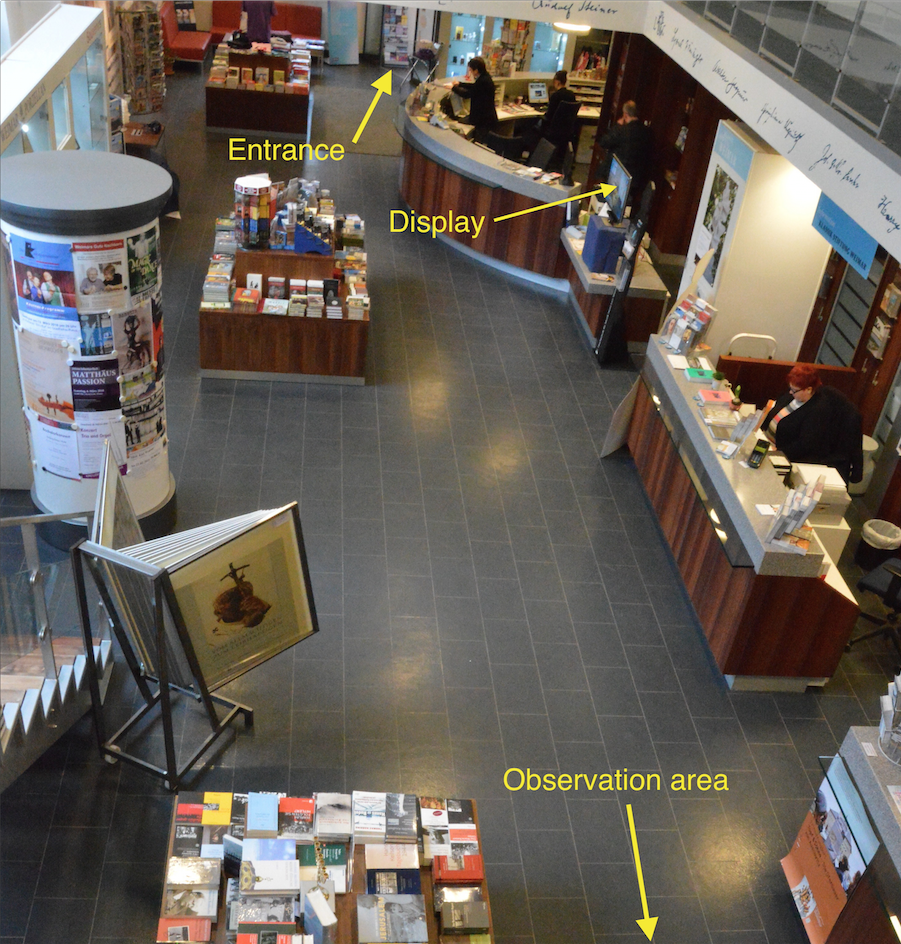
\includegraphics[width =0.8\textwidth,height=8cm]{Figures/8/tourist_info}%
    \caption{Weimar Tourist Information Center Top-view picture, The locations are marked with yellow arrows.}%
    \label{fig:Tourist_info_center}%
\end{figure}


\subsection{Duration}
Each of advertisement condition was installed for five days in the following three weeks.

\begin{table}[H]
\caption{Week sequence}
\label{tab:advertisementWeeks}
\centering
\begin{tabular}{l c c c }
\toprule
\tabhead{Advertisement} & \tabhead{1st Week} & \tabhead{2nd Week} & \tabhead{ 3rd Week} \\
\midrule
\textbf{Non-Interactive}     &   X    &         &     \\
\textbf{Body Interactive}     &        &    X    &    \\
\textbf{Mobile Interactive}  &        &         &   X   \\
\bottomrule\\
\end{tabular}
\end{table}



\subsection{Internal Validity}
To be confident that the change in the weeks would not effect the findings, 
extra effort was done to make all the week environmental conditions the same as much as possible. The screen was installed in the same location, had the same screen brightness, height and also the surroundings of the screen were not altered, we asked the responsible person in tourist information center not to change anything in the surrounding. The luck was also with us that almost the weather conditions were the same too, but the only thing we could not control was the number of passerby; The flow of passers-by were also be nearly the same.


\subsection{Participants}
The participants were the ones who pass by the screen, none of the participants were informed about this study nor any notes were put at the entrance. Roughly \%60 of the participants were elder aged between 30-60, \%25 were young and the rest \%15 were children.


\subsection{Data gathering}
Several types of data from different aspects were gathered for each individual week to be able for analyzing and also be able to answer new arising questions after the onsite evaluation, the bellow types of data were gathered.


\begin{enumerate}
\item \textbf{On-Site Observation} \\
Observation periods were arranged in two different time slots per day, the first time slot was from 10:00 – 12:00 and the second was from 14:00 – 16:00, except for Saturday and Sunday where the tourist information center was open only until 14:00, then the observation period was from 10:00-12:00 and 13:00-14:00. During these two time slots the bellow observations were made and to remove the effects of specific time order,the orders were counterbalanced.

\begin{enumerate}
\item \textbf{Attention Level measurement} \\
Attention level is how much a person gives attention to the display, which consist of number of glances and number of ignores and how long a person is standing infront of the display. At the beginning gaze-tracking method was considered for accurate measurement of attention level, a very impressive work have been done from Intraface \cite{Intraface} that can not only detect glances but also human emotions at the time, but because of high flow rate that method was not used and instead the glance counting which was proposed by \cite{glancingcount} that has formalized a ranking system from which  glance is considered if a person reacts to the display by turning his/her head toward it that last less than 3 seconds.

One hour attention level counting for each time slot was conducted, in which the observer was writing the number of people passing by and how many of them glanced and ignored the screen.see the glance counting sheet in Appendix: \ref{AppendixA}.1


\item \textbf{Passers-by behavior and Interviews} \\
During one hour per time slot per day the passerby behavior were observed like how they approach to the screen, how do they react, and what are they looking for and even how they ignore the display and after they are done with the display engagement a very short interview was taken from them. 

Interviews were taken from the passerby that had some sort of engagement with the display like for non-interactive advertisement the people were interviewed that they stood for a while and saw the advertisement and for the interactive advertisement the people were interviewed that interacted or tried to interact with the system.
A leaflet, that describes the thesis goal and interview consent form was handed to the participants and after signature the interview was conducted. All the interviews were audio recorded and later transcribed for analysis, all interviews took in average 4 minutes, the reason we took short interviews was that most of the people were tourists and had little time to stay and even some of them rejected interview because of shortage of time.
Each week there were some variation in the questions dependent to the type of advertisement.  
%See appendix \ref{AppendixD}.1
\hilight{fix the appendix}


\end{enumerate}


\item \textbf{System Logs} \\
The Advertisement application can generate the bellow logs.
\begin{enumerate}
\item	\textbf{Non-Interaction application} \\
Only duration(seconds) spent in front of the display is logged for each individual person.

\item	\textbf{Interaction application}\\
For this type the system can detect

\begin{itemize}
\item	Time user joins.
\item	Interaction completion time.
\item	Number of tasks (locations) explored.
\item	Whole duration spent(sec).
\item	If the user has seen advertisement or not.
\end{itemize}

\end{enumerate}

\item \textbf{Colored-image recording} \\
Colored-image recording from Kinect camera was done during entire three weeks for non-interactive and interactive advertisement for many reasons.

\begin{itemize}

\item Passers-by engagment measurment \\
As discussed earlier, engagement was defined as involvement of audience with the display. The passers-by were considered as engaged if they had stayed longer than 3 seconds, in this sense two types of data were gathered for engagement.

        \begin{itemize}
        \item Number of engagements. \\
        Meaning how many people were engaged.

        \item Engagement duration. \\
        How long audiences were engaged with the system.

        \end{itemize}

\item Count the number of Honeypot effects and landing effects.
\item Match the log data with the video data for accuracy.
\item Observe passerby behavior in detail.
\end{itemize}

Because of limited space and processing power, the actual depth information (x,y,z) for individual points was not stored but a 2D colored image was taken per second and after the image recording was done, in lab another post processing script was applied to integrate a static background using Adobe Photoshop application. To match the data logs and the image frames each image name consisted the date and time as (10.12.43.21.png).


\begin{figure}[H]
    \centering
    \begin{subfigure}[H]{0.45\textwidth}
        \centering
        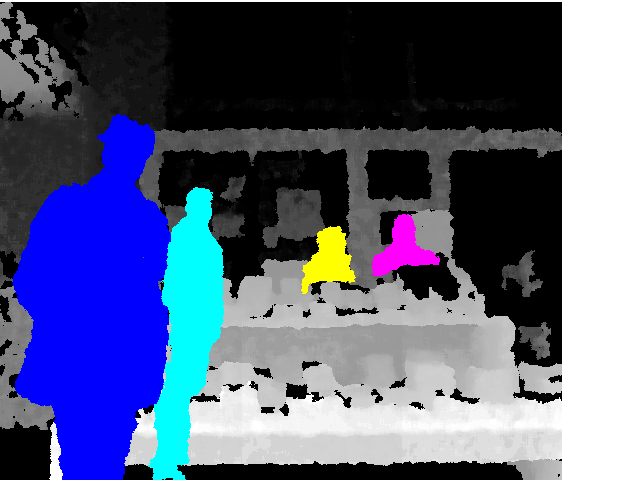
\includegraphics[width=\textwidth,height=4cm]{Figures/8/d1}
        \caption{}
        \label{fig:d1}
    \end{subfigure}
    \begin{subfigure}[H]{0.45\textwidth}
        \centering
        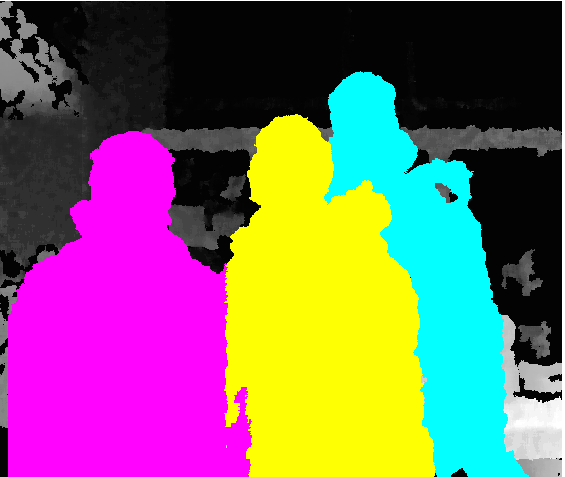
\includegraphics[width=\textwidth,height=4cm]{Figures/8/d2}
        \caption{}
        \label{fig:d2}
    \end{subfigure}
    \caption{Depth recording examples}
    \label{fig:DepthRecordedImages}
\end{figure}




\end{enumerate}

Other pictures were also taken using mobile phone from the scene, verbal permission were taken before the photographing them.


\section{Data Analysing}
\subsection {Glance counts} 
The glance counts were transformed from paper to spreadsheet in which number of glances and ignores were recorded individually and then combined from which mean value and percentages are extracted.
 \hilight{fix appendix}
 %see Appendix \ref{AppendixD}.2, \ref{AppendixD}.3 and \ref{AppendixD}.4 for each week.

\subsection {Interviews} 
All the interviews were transcribed and color coded from which interesting categories had emerged, each code is separately discussed in the finding section, To see color coded diagram see Appendix
 \hilight{fix appendix}

 %\ref{AppendixD}.5, \ref{AppendixD}.6 and \ref{AppendixD}.7 for each week. 

\subsection {Display Engagement phases and time} 
Log files along depth images were seen and compared to have accurate values for each engagement phases and the whole interaction phases. depth frames were manually frame-by-frame analysed and the logs were cleared from any possible mistakes.

\subsection {Honeypot and landing effects}
These two effects were observed mainly from the depth frames and also partially from onsite observation.

\subsection {Other observations}
The observations were done onsite, the observer wrote down any important event happened at that moment, These notes also include observer own point of view of understanding the scenario during the entire day and week. Most of the notes have time stamp. See Appendix
\hilight{fix appendices}
%\ref{AppendixD}.8, \ref{AppendixD}.9, and \ref{AppendixD}.11.\\
The depth recordings were also observed frame-by-frame to see anything that was missed when the observer was not present at the center. Different behaviors are extracted from the observation, which you will find in findings.


\section{Findings}
To be more precise and structured, I have divided the finding sections in two separate sub sections, the first section describes the findings from each condition (Non-interactive, Body interactive and mobile interactive) separately and the second section compares the findings of these conditions among each other.


\subsection{Non-Interactive findings}

\begin{enumerate}

\item \textbf{Attention Level measurements} \\
The number of glances and ignores were measured for the five consecutive days as shown bellow, each day (bar) has less than half number of glances compared to number of ignores and in total the average glance is \%28, which slightly corresponds above (1/4) portion of passers-by.


\begin{figure}[H]
    \centering
    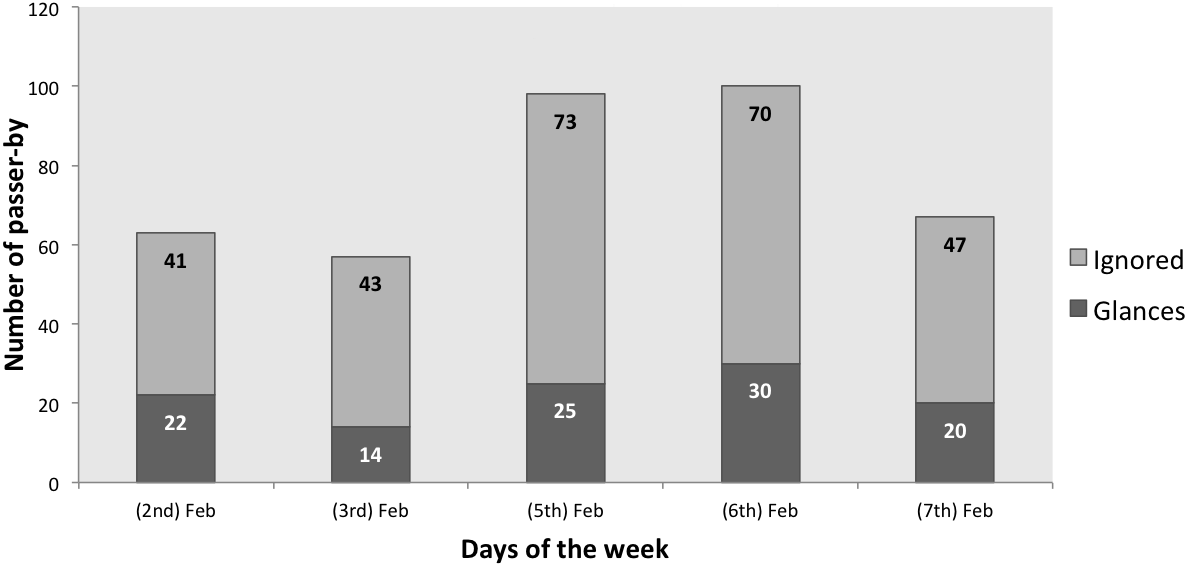
\includegraphics[width=0.8\textwidth,height=6.5cm]{Figures/8/non_inter_findings/Non_Inter_chart}%
    \caption{Non-interactive attention level chart}%
    \label{fig:Nonattentionlevelchart}%
\end{figure}


\begin{figure}[H]
    \centering
    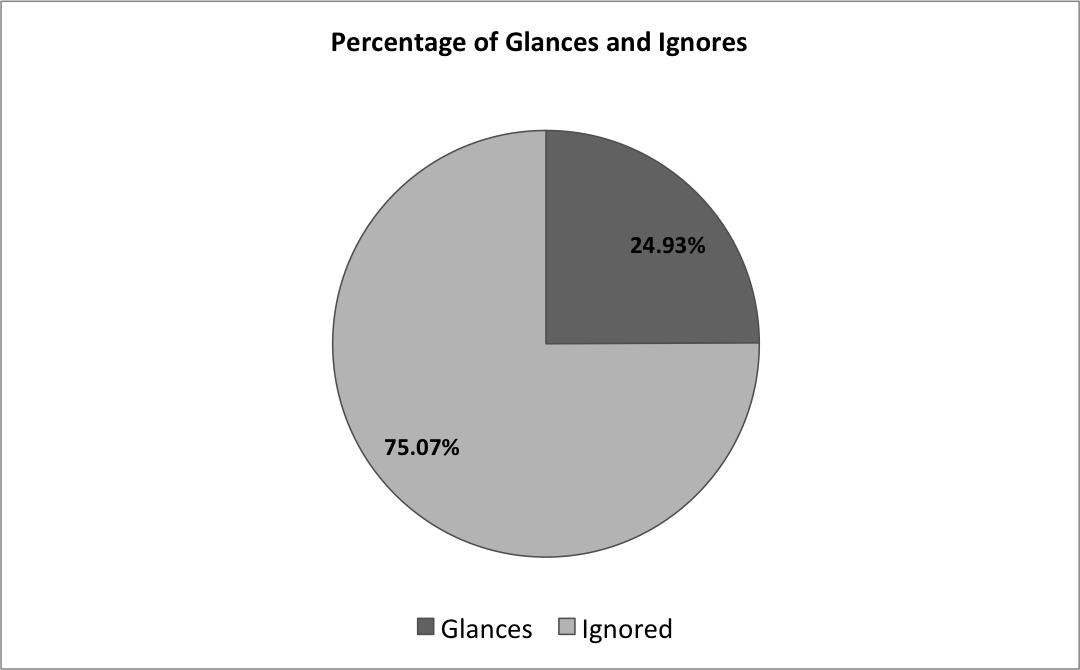
\includegraphics[width=0.45\textwidth,height=6.5cm]{Figures/8/non_inter_findings/non_inter_percentage}
    \caption{Non-interactive Attention level percentage}%
    \label{fig:Nonattentionlevelpercentage}%
\end{figure}



\item \textbf{Engagement Time} \\
Not all people would take time to see the advertisement, some participants took very little time like 4-5 seconds and some also saw the ad for about 100 seconds, which is almost twice of the advertisement time, so dependent to the interest, people were engaged in different durations and in average it took about 34 seconds to be engaged.


\item \textbf{Number of engaged passers-by} \\
Counting the entire passers-by was a challenge and there was not accurate and automated method to do, therefor each day’s recordings were watched and the numbers of passers-by were counted manually, this intense work was carried out with a couple of computer science students who voluntarily participated.  
The bellow chart shows all the count of passers-by and out of those the people who were stood in front of the screen for more than 3 seconds were flagged as an engaged passer-by.



\begin{figure}[H]
    \centering
    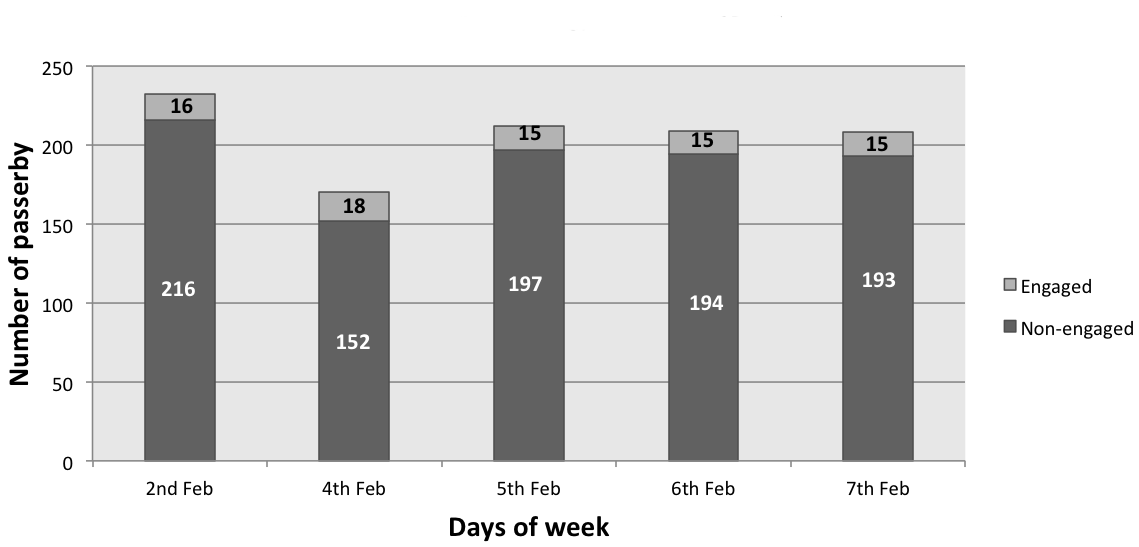
\includegraphics[width=0.8\textwidth,height=6.5cm]{Figures/8/non_inter_findings/non_inter_engage_day}
    \caption{Non-interaction Number of engaged and Non-engaged passers-by}%
    \label{fig:Nonengagedandengagedby}%
\end{figure}

\begin{figure}[H]
    \centering
    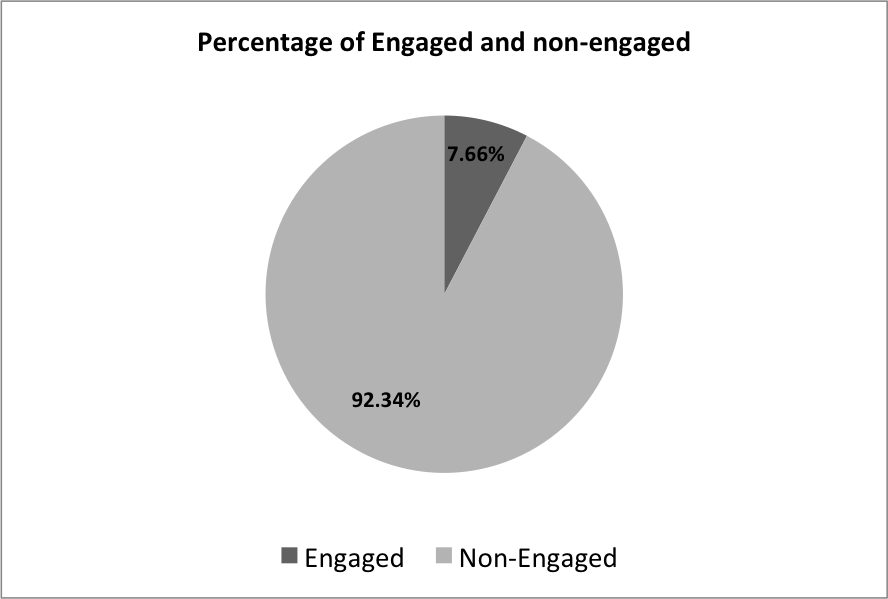
\includegraphics[width=0.5\textwidth,height=6.5cm]{Figures/8/non_inter_findings/non_eng_percentage}
    \caption{Percentage of engaged and Non-engaged passers-by}%
    \label{fig:Nonengagedpasserbypercentage}%
\end{figure}


As can be seen in above chart it shows the number of passers who were engaged and number of passers-by who did were not engaged. The chart shows very few engaged people for each day and as an average \%7.66 of the whole population was engaged within 5 days.


\end{enumerate}


\newpage
\begin{enumerate}
\setcounter{enumi}{3}
\item \textbf{Landing and Honeypot effects}
\end{enumerate}

\begin{wrapfigure}[20]{R}{0.3\textwidth}
  \vspace{-20pt}
  \begin{center}
    \includegraphics[width=0.30\textwidth,height=90mm]{figures/8/non_inter_findings/effects/landing}
  \end{center}
  \vspace{-20pt}
  \caption{Landing effect}
  \vspace{20pt}
\end{wrapfigure}
Some might argue that Landing\cite{EnticingPeople} effect do not exist in non-interactive displays because the displays do not react suddenly when a user pass by the screen, but at the same time users may react to the visual stimuli that generated by the non-interactive advertising by showing random contents, which is by its nature independent to the people around.

In non-interactive the silhouette is not projected and the passers-by do not see themselves in the screen, but still for some other reasons passers-by turned back from the end of the screen to the middle of the screen, there could be many reasons behind this, (1) maybe the screen was showing the advertisement video in which pages are changing after one another, (2) maybe the screen was showing city map in which interest locations are animated, (3) beside visual any other personal interest has dragged passers-by toward the screen. 

As can be seen in the figure in the right, in frame (A) a person passes-by the display and is almost crossing the display, but suddenly in frame (B) he notices something and he stops, in frame (C) he explicitly shows his reaction by turning back toward display and in frame (D) he comes closer to the screen and starts to see or read advertisement content. \\


\begin{wrapfigure}[17]{L}{0.3\textwidth}
  \vspace{-20pt}
  \begin{center}
    \includegraphics[width=0.30\textwidth,height=90mm]{figures/8/non_inter_findings/effects/honeypot}
  \end{center}
  \vspace{-20pt}
  \caption{Honeypot effect}
  \vspace{-60pt}
\end{wrapfigure}
Honeypot\cite{LookingGlass} effects in non-interactive displays are rare because they do not make passers-by become curious about themselves, and passers-by do not perform any interaction or react differently, that could be noticed by other passers-by, therefor most of the observations on this effect seemed to be more passive and this effect could be due to that a friend was watching the screen and another friend of him / her got attracted or attracted person might just had another intension for-example to talk him. The scenarios seemed to be very personal.

As can be seen in the picture in the left, In frame (A) a lady is standing in front of the monitor and reading the content and after a while in picture (B) another person is approaching the monitor to see what was happening and immediately another person in picture (C, D) was also attracted to come close and see what was going on. 


The bellow the number of effects that occured for each day is recorded.

\begin{minipage}{\textwidth}
\begin{flushright} 
\begin{table}[H]
\caption{Landing and honeypot effects}
\label{tab:landingandhonypot}
\centering
\resizebox{6cm}{1cm}{
\begin{tabular}{| l | c | c |}
\toprule
\tabhead{Days} & \tabhead{Landing effect} & \tabhead{Honeypot effect} \\
\midrule
\textbf{2nd Feb}  & 1 &  1 \\
\textbf{4th Feb}  & 0 &  1 \\
\textbf{5th Feb}  & 2 &  3 \\
\textbf{6th Feb}  & 0 &  3 \\
\textbf{7th Feb}  & 1 &  1 \\
\bottomrule
\end{tabular}
}
\end{table}
\end{flushright} 
\end{minipage}



\begin{enumerate}
\setcounter{enumi}{4}

\item \textbf{Interview} 
\begin{enumerate}
\item Likes \\
Many things from the advertisement were interesting, like the concept of map and the design. As one stated that, ``\emph{I find the idea good, it is nice to see the pictures of the places on the map}'', ``\emph{it is very nice idea because it will be remembered and when I go to the city I will remember}''

\item Dislikes \\
Most of the respondents complained on the speed of the advertisement that how fast the image changes as one said ``\emph{But the pictures were changing very fast}'' other said, ``\emph{advertisement is a little fast}'' They mentioned that why speed is an issue as stating, ``\emph{we wanted to see the map}'', ``\emph{ Could not read the text}''. Many things were disliked by some of the respondents like the advertisement theme, one said, ``\emph{It did not have Bauhaus Theme, the color and that design}'' One respondent also disliked the blinking points.

\item  Participation \\
Respondents mentioned the same excuses that were given at body interactive advertisement, one said, ``\emph{I will join if I am free}'', other said, ``\emph{I have no time}'', or ``\emph{if the weather is good}''. 

\item  Advertisement recall \\
People could recall the ad, as one mentioned, ``\emph{It is for a tour of Bauhaus in Weimar}'' other said, ``\emph{People can visit the city}'' and some mentioned directly the name of the program ``\emph{Bauhaus-Spaziergang}''.

\item Recommendations \\
There were many recommendations proposed by the responders, which was on content, speed, design.Content related recommendations was that one said, ``\emph{If the prices are mentioned it would be good so that they can decide if they want to take it or not}'' other said on timing, ``\emph{how long does this tour take so people arrange their}''. Another mentioned on speed like ``\emph{it must be little slow}''.

\end{enumerate}


\item \textbf{Audience behaviors} \\
Note taking technique and video observations helped to analyze the environment and behavior of people around the display. 
See appendix  %\ref{AppendixD}.8
\hilight{fix this appendix}

\begin{itemize}

\item Passive: \\
The behavior toward non-interactive during the 5 days observation seemed to be very calm and passive, passers-by selectively came to watch the screen there was no curiosity nor attractiveness that had driven their attention. It was thread as a source of information and whenever they approach the screen the participants would normally stand for a very short time and after looking for 1-2 pop-up pictures on the screen they would leave, except for participants that was looking for some events that stood for the complete duration of the advertisement.There was an interactive object in front of the display on the table, which many people tried to play.


\item Display negligence  \\
At most of the occasions the display was neglected and passers-by were busy with their own personal activities and discussions even though they were standing in front of the display facing toward it.

\item Display blindness \\
Passers-by also ignored and passed by the display because they did not expect to be something special related to them.

\item Display as information board \\
Some of the passers-by expected the display to be a source of information, for example some tourist stood in front of the display to see the map and find out locations by reading the street names on the map.

\end{itemize}


\end{enumerate}

\begin{figure}[H]
    \centering
    \begin{subfigure}[H]{0.32\textwidth}
        \centering
        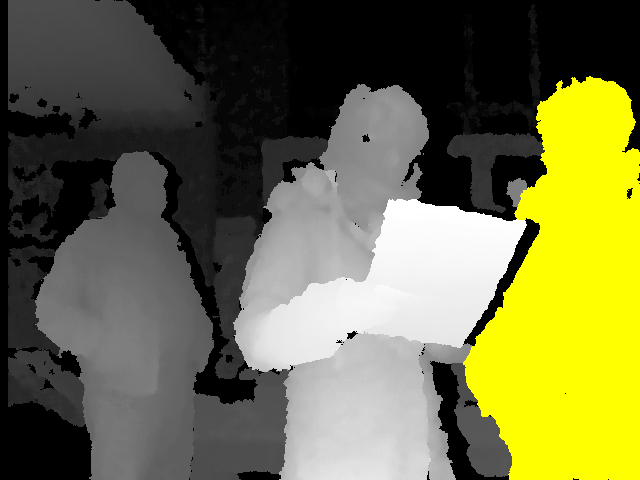
\includegraphics[width=\textwidth]{Figures/8/non_inter_findings/effects/neglegance}
        \caption{}
        \label{fig:non-blindness}
    \end{subfigure}
    \begin{subfigure}[H]{0.32\textwidth}
        \centering
        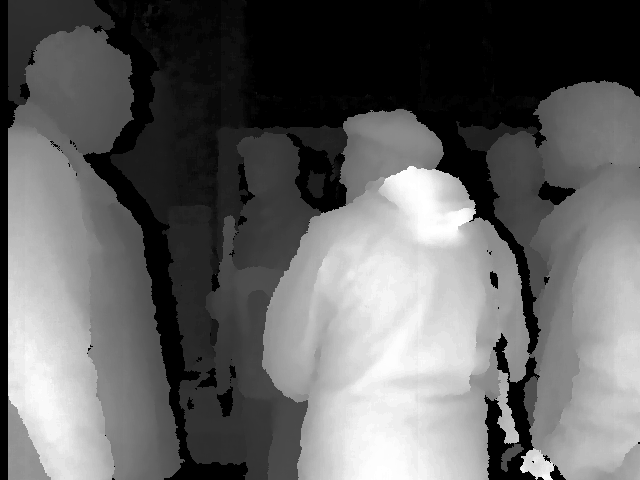
\includegraphics[width=\textwidth]{Figures/8/non_inter_findings/effects/displayblindness}
        \caption{}
        \label{fig:non-negligence}
    \end{subfigure}
    \begin{subfigure}[H]{0.32\textwidth}
        \centering
        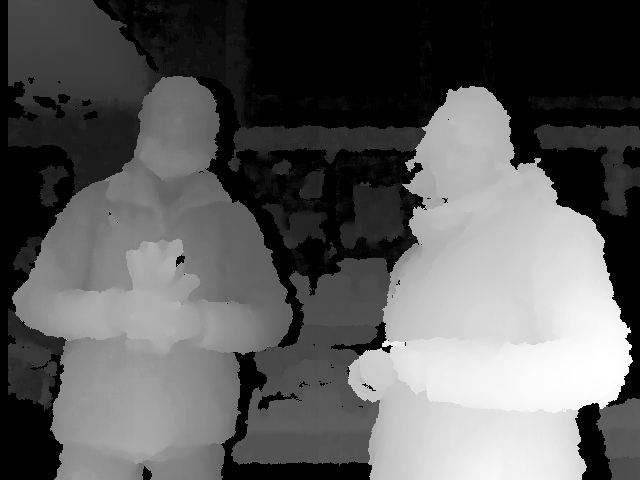
\includegraphics[width=\textwidth]{Figures/8/non_inter_findings/effects/reading}
        \caption{}
        \label{fig:non-reading}
    \end{subfigure}
    \caption{Passers-by Behaviors}
    \label{fig:three-non-behavior}
\end{figure}

As can be seen above, the first two pictures show that the display is completely ignored and people are busy with themselves. Picture C shows two couples are reading the screen.

\subsection{Body Interactive findings}

\begin{enumerate}
\item \textbf{Attention Level measurements} \\
The bellow chart shows the observation number of glances and ignores of passers-by for two distinct hours of five days. As can be seen the in most days the number of glances and ignores are almost near but not still ignores percentage is higher, as can be seen in the pie-chart \%41.41 are the number of glances and around \%59 is the number of ignores. 
\begin{figure}[H]
    \centering
    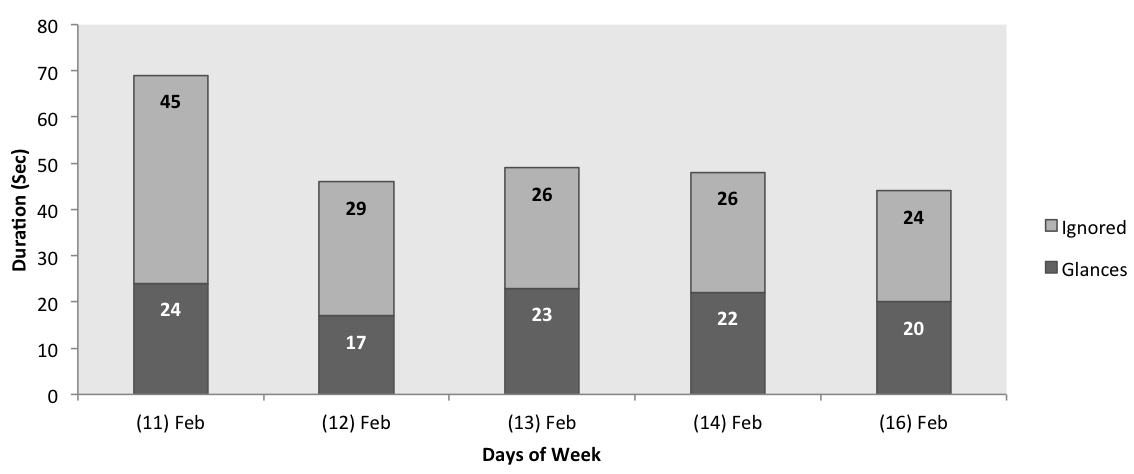
\includegraphics[width=0.9\textwidth,height=6.5cm]{Figures/8/body_inter_findings/Body_Inter_chart}%
    \caption{Attention level chart}%
    \label{fig:bodyattentionlevelchart}%
\end{figure}


\begin{figure}[H]
    \centering
    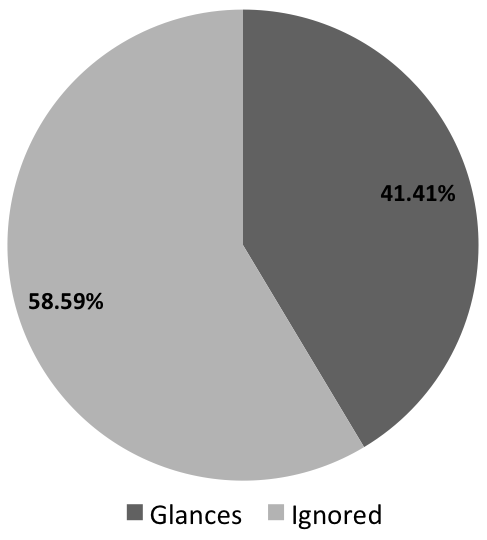
\includegraphics[width=0.45\textwidth,height=6.5cm]{Figures/8/body_inter_findings/body_inter_percentage}
    \caption{Body interactive Attention level percentage}%
    \label{fig:bodyattentionlevelpercentage}%
\end{figure}



\item \textbf{Engagement phases and time} \\
\hilight{take average of single and group interaction time}\\
There were passers-by who were very interested in the interaction that played the game even three times, some people triggered the game and left in the middle and some people were just staring at the screen and did not triggered the game, therefor people were engaged in different stages of the game and spent between (10, 200) seconds, and in average passers-by spent around 42 seconds.

\begin{figure}[H]
    \centering
    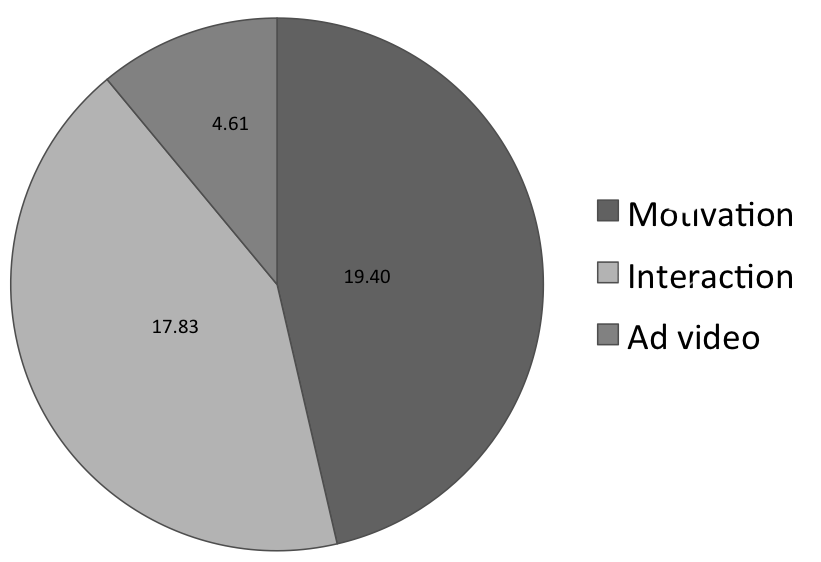
\includegraphics[width=0.6\textwidth,height=6.5cm]{Figures/8/body_inter_findings/body_avg_phases}
    \caption{Average time for each phase}%
    \label{fig:bodyaveragephases}%
\end{figure}

The advertisement was divided in three main section (1) Attention / Motivation, which is the pre-interaction phase that the participant has not started the game and just playing with body or looking to the screen or reading call-to-action text, in this stage some people by just looking to the screen approached and started the interaction less than 5 seconds and some people took longer time to think and then triggered the game, at some occasions participants just left without triggering the game so in average it took around 20 seconds for this stage. (2) The interaction part in which people again took different times, some people played more than two or three times and some played the first element and left so in average it took about 18 seconds for this stage. (3) The advertisement video which had the least time spent most of the participants left the screen after they saw the advertisement video in 2 seconds and some were excited to play again so they waited for a while In front of display until the end of advertisement video this was very rare among participants, so in average it took around 4.5 seconds for advertisement video.


\item \textbf{Number of engaged passers-by} \\
As mentioned before, for non-interactive the entire day’s recordings were manually analyzed frame by frame from which the number of passers-by were counted. The bellow chart shows all the count of passers-by and out of those the people who stood in front the screen for more than 3 seconds were flagged as an engaged passer-by.

\begin{figure}[H]
    \centering
    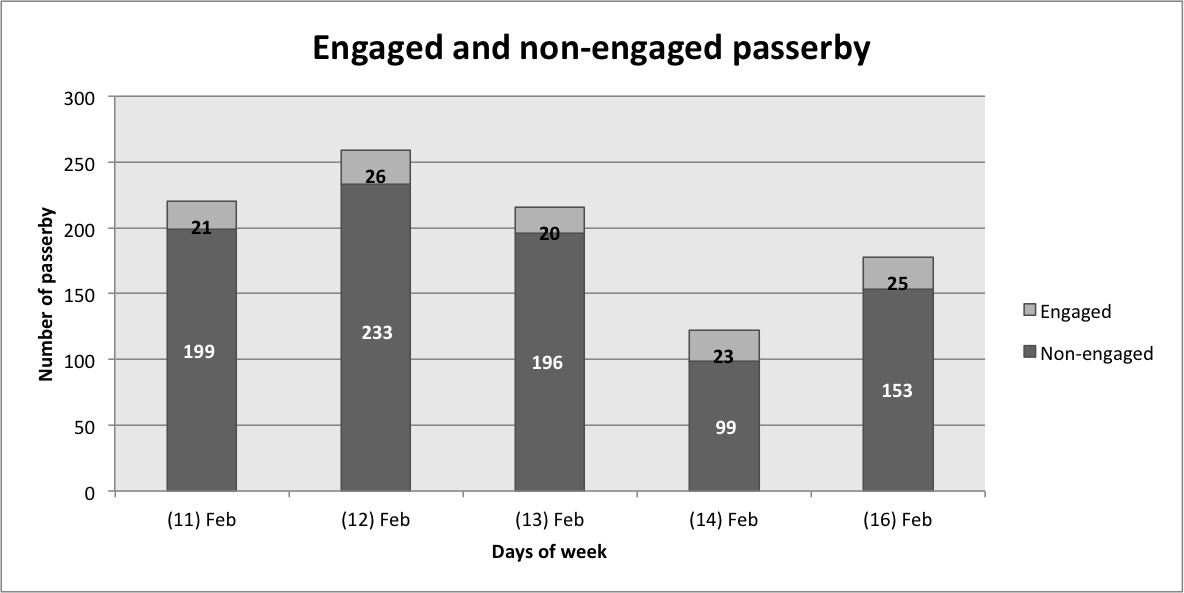
\includegraphics[width=0.8\textwidth,height=6.5cm]{Figures/8/body_inter_findings/body_inter_engage_day}
    \caption{Body interactive Number of engaged passerby}%
    \label{fig:bodyengagedandengagedby}%
\end{figure}

As can be seen from the chart bellow the number of them are shown in bar chart for each of the day. And in average around \%12 of the passers-by were engaged with the screen. 

\begin{figure}[H]
    \centering
    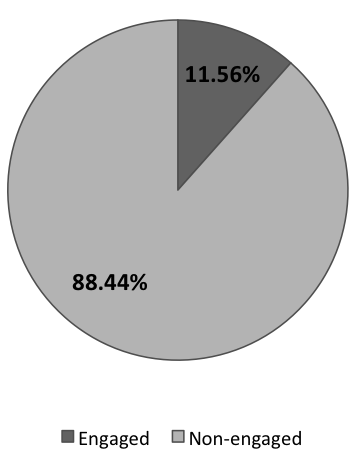
\includegraphics[width=0.4\textwidth,height=6.5cm]{Figures/8/body_inter_findings/body_eng_percentage}
    \caption{Percentage of engaged and non-engaged passers-by}%
    \label{fig:bodyengagedpasserbypercentage}%
\end{figure}


\end{enumerate}


\newpage
\begin{enumerate}
\setcounter{enumi}{3}
\item \textbf{Landing and Honeypot effects}
\end{enumerate}

\begin{wrapfigure}[23]{r}{0.3\textwidth}
  \vspace{-60pt}
  \begin{center}
    \includegraphics[width=0.3\textwidth,height=120mm]{figures/8/body_inter_findings/effects/landing}
  \end{center}
  \vspace{-20pt}
  \caption{Landing effect}
  \vspace{-10pt}
\end{wrapfigure}
Interactive displays are known from the most well known user behaviors, (1) honeypot effect and (2) landing effect because they drag passers-by attention significantly so that the passers-by be involved. In body interaction both of these effects were observed while direct observation and while depth recording analyzing. This was the most time consuming task ever and took about a week to analyze and document them.

As before landing effect was discussed, that a person recognizes the interactivity after he /she has already passed by the screen and as a result walks back to confirm if the interactivity is there and check what the display is about, and how to interact. In body interaction all of the landing effects has happened by noticing their silhouette on the screen and has turned back, these effects were observed for individual and group passers-by.

As can be seen in the picture in the right, in the first frame two persons are passing by the screen and one of them has not seen his self in the display even his silhouettes was projected, but the second person who has yellow color (A) notices the interactivity while his friend is still continuing to pass (B, C), but this guy who has noticed stops (colored changed by Kinect camera) in frame (C, D), his stopping drags his friend attention and at this point his friend notices the display and walks back to see his self in the screen (E).


\begin{wrapfigure}[20]{l}{0.3\textwidth}
  \vspace{-20pt}
  \begin{center}
    \includegraphics[width=0.3\textwidth,height=100mm]{figures/8/body_inter_findings/effects/honeypot}
  \end{center}
  \vspace{-20pt}
  \caption{Honeypot Effect}
  \vspace{-20pt}
\end{wrapfigure}
The honeypot effect is the effect, which other people are attracted by noticing the current people that are somehow involved (interacting) with the display. The people by whom the honeypot effect had occurred, were different, some people might have been in the initial interface by just playing with their silhouette, or they were actively interacting with the game or they were watching the advertisement video, that dragged the people’s attention. The engagement duration was higher, as a result participants stood longer, which results in higher number of honeypot effects.

As can be seen in the picture on the left, a boy is interacting with the system in frame (A), the body moves a bit behind from the display in frame (B) at this time another random person who does not know him notices him or has noticed before, tries to approach to the screen in frame (C) and then when the person sees his silhouette then he tries to actively to take control of the interaction by coming in the center of the screen in frame (D) and the other active person was left behind the scene.

The bellow chart lists all the frequencies of honeypot effect and landing effects that was recorded from the depth recordings and onsite observations. \\



\begin{minipage}{\textwidth}
\begin{flushright} 
\begin{table}[H]
\caption{Landing and honeypot effects}
\label{tab:landingandhonypot_body}
\centering
\resizebox{6cm}{1cm}{
\begin{tabular}{| l | c | c |}
\toprule
\tabhead{Days} & \tabhead{Landing effect} & \tabhead{Honeypot effect} \\
\midrule
\textbf{11 Feb}  & 2 &  2 \\
\textbf{12 Feb}  & 3 &  3 \\
\textbf{13 Feb}  & 2 &  2 \\
\textbf{14 Feb}  & 2 &  5 \\
\textbf{16 Feb}  & 3 &  3 \\
\bottomrule
\end{tabular}

}
\end{table}
\end{flushright} 
\end{minipage}


\begin{enumerate}
\setcounter{enumi}{4}
\item \textbf{Interviews} \\
The interviews were coded each individually and as a result the bellow categories are extracted, these categories are mainly taken from the questions and others are from the replies of the participants. 

\begin{enumerate}

\item Noticing \\
    Different people had their different experience and reaction when they noticed themselves in the display for the first time. Some of the people were standing and looking some books for long time when they saw themselves and for confirmation they waved toward the screen, as one said ``\emph{Yes at first I thought that it is not me. I waved my hand and came near.}'' Other said, ``\emph{Yes I saw my blue color body}''. Other participants noticed at the time of passing from front of the screen, ``\emph{when I was passing I saw myself in the screen.}'' Other people saw their friend first then noticed themselves like one said, ``\emph{I saw my friend in the screen and came near and I was also there with blue color.}'' One participant who usually comes to the center every week said that because the screen was newly installed I came near to the screen to see what is new inside.

\item Ad recall \\
    Respondents responded accurately the content and goal of the advertisement as one said, ``\emph{It was about a tour of Bauhaus, Bauhaus Spaziergang.}'' ``\emph{It was about tour in the city.}'' And other said, ``\emph{It was about Bauhaus-Walk. City tour.}'' And other said, ``\emph{it is something to do with Bauhaus city walk}''.

\item Interest \\
    People find this type of interaction very interesting, funny and motivative, one participant mentioned that, ``\emph{I liked to see myself in the screen, it was funny.}'' Other says the use of media is very interesting and comfortable for people, ``\emph{I think that the people with the use of media is comfortable}''. The use of this type of interactive advertisement give people some sort of good feeling toward Bauhaus-Walk event like one said, ``\emph{Bauhaus is very interested to me and it sounds fun}''. People also liked the way content was inside the advertisement like one said, ``\emph{It is very interesting to see the pictures}'' and even one participant exactly mentioned the goal of the advertisement interaction, ``\emph{it was a very interesting idea and it is like a small interactive tour for the people who want to take Bauhaus-Walk.}''

\item Event participation  \\
    Respondents showed sign of interest to join the program in future but are not able to join quickly because of many reasons like they are here for short visit as one said, ``\emph{We are here in Weimar for short visit}'', others said they are busy with many other programs like one said, ``\emph{Now we are going to Weimar Museum}''.

\item Confusions \\
    There was some confusion during interaction, like the interaction seemed unclear, one said, ``\emph{I did not understand how it works}'' other said, ``\emph{I left because I did not understand}'' and some people also experienced this by coming very close to the screen and nothing is shown to them at that time, ``\emph{when I was standing I saw that it says come near, and I came near to the screen and the map came but I left after standing for a short time because I did not understand it.}''

\item Dislikes \\
    When a person hovers on a location in the map, a related picture is shown on the screen and deems off after a while, some participants complained about time and said, ``\emph{Pictures goes very fast}'', one person complained about the rendering speed and said, ``\emph{Pictures come very late}''.

\item Recommendations  \\
    Respondents recommended that the advertisement should be able to hint users on how to use it, as one said, ``\emph{It would be good to put some more information that how we can use it.}''  Other said that ``\emph{Maybe explain how someone can walk with these body figures}''. One person even said, ``\emph{It is good that here someone stand and describe it to the people who come near to the screen.}'' Some of the participants also recommended to slow down the picture changing of the advertisement.
\hilight{fix the appendix}
%check appendix \ref{AppendixD}.9 and \ref{AppendixD}.10

\end{enumerate}

\item \textbf{Other observations} \\
During the body interactions despite honeypot and landing effect other different kinds of behaviors have been observed and how passers-by reacted when there was an interactive display, the behavior with the display was much different compared to non-interactive as listed bellow.

\begin{itemize}
\item Group and individual interactions: \\
Passers-by interacted both in groups and individual, the groups ranged from two to four people. \%49 of engagement happened by individuals and \%51 engaged were done in groups. 
 The bellow pictures show different group interactions happening between friends as in picture (A, B) and another three persons interacting in picture (C, D).

\begin{minipage}{0.89\textwidth}
\begin{flushright}
\begin{figure}[H]
    \centering
    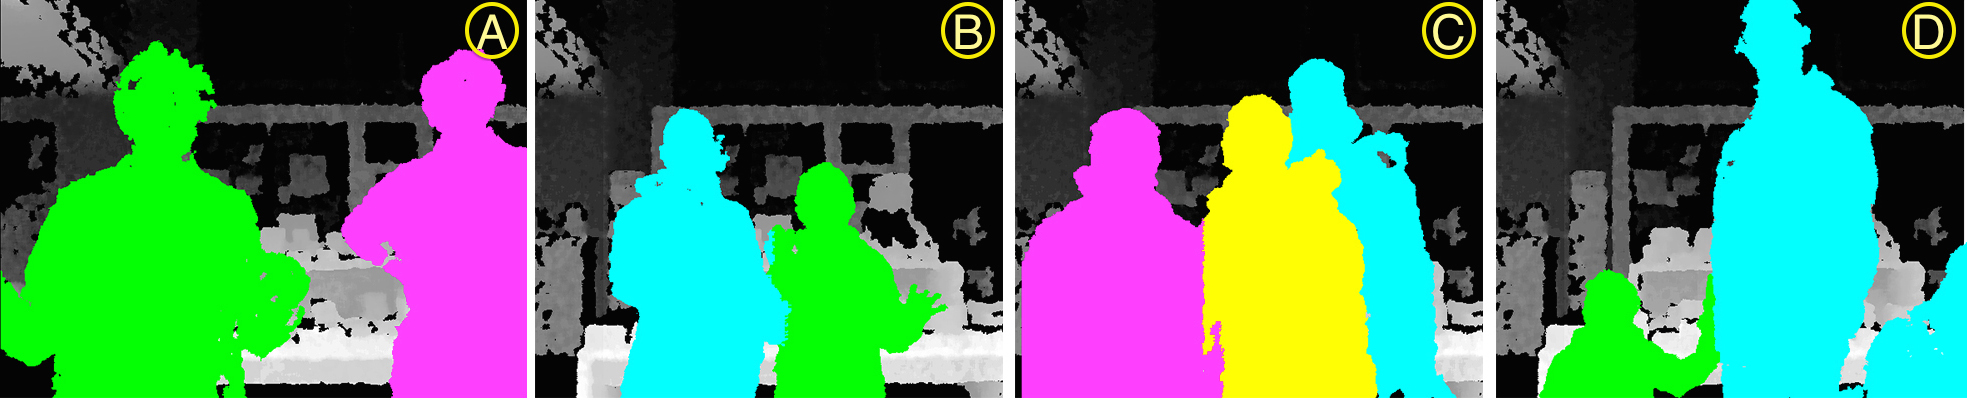
\includegraphics[width=\textwidth,height=30mm]{Figures/8/body_inter_findings/effects/group}
    \caption{Group interactions}
    \label{fig:group_interaction}
\end{figure}
\end{flushright}
\end{minipage}


%The bellow chart shows the percentage of group and individual interactions during five days. 

%\begin{figure}[H]
%    \centering
%    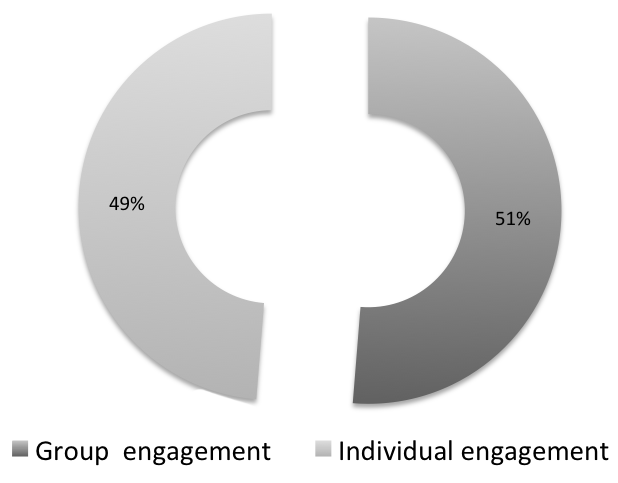
\includegraphics[width=0.3\textwidth,height=3.5cm]{Figures/8/body_inter_findings/group_individual_interaction}
%    \caption{Group and individual interactions.}%
%    \label{fig:groupsinglebodyengagedpasserbypercentage}%
%\end{figure}




\item Calling others: \\
People were getting really excited and liked to call his / her friends to come and join and have fun with the interaction, most of this reaction was seen between children and parents and couples. As can be seen in frame (A) a person is watching the display and then moves out in frame (B) and in frame (C) calls a friend of him/her and in frame (D) both of them are in center of the screen and watching themselves in it.

\begin{minipage}{0.89\textwidth}
\begin{flushright}
\begin{figure}[H]
    \centering
    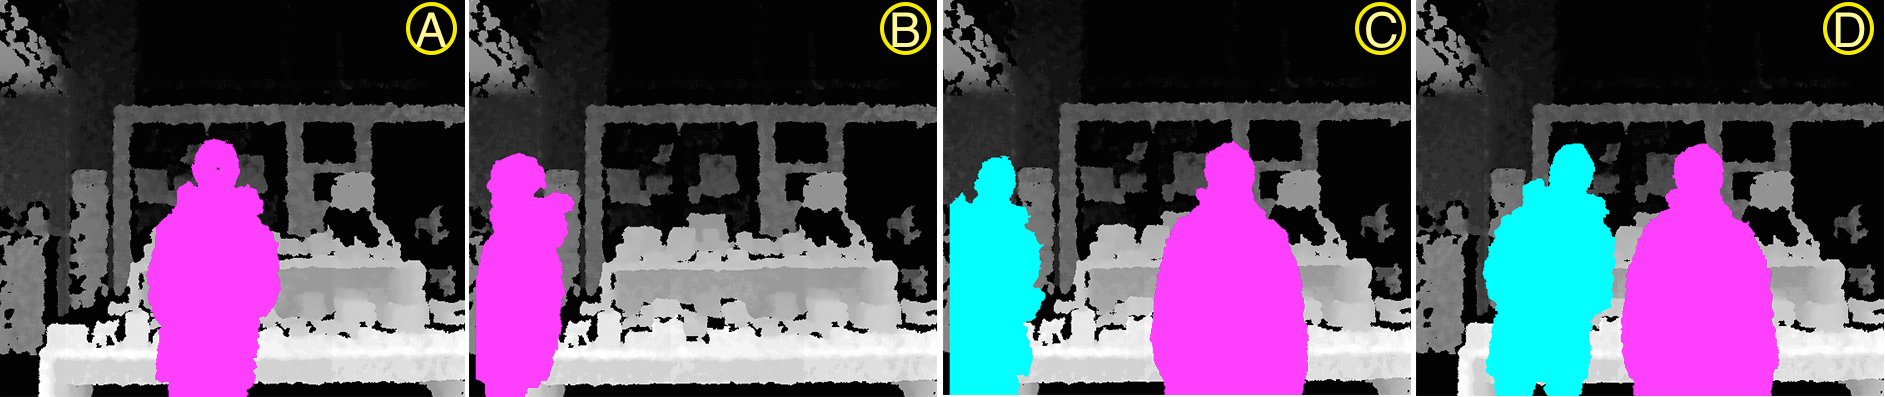
\includegraphics[width=\textwidth,height=30mm]{Figures/8/body_inter_findings/effects/calling_others}
    \caption{Calling others}
    \label{fig:calling_interaction}
\end{figure}
\end{flushright}
\end{minipage}


\item Playing with silhouette:  \\
Passers-by liked the different colors specially when they were couples or children before they triggered the interaction. As can be seen in bellow picture there is a couple that likes to play with the different colors of their silhouette.

\begin{minipage}{0.89\textwidth}
\begin{flushright}
\begin{figure}[H]
    \centering
    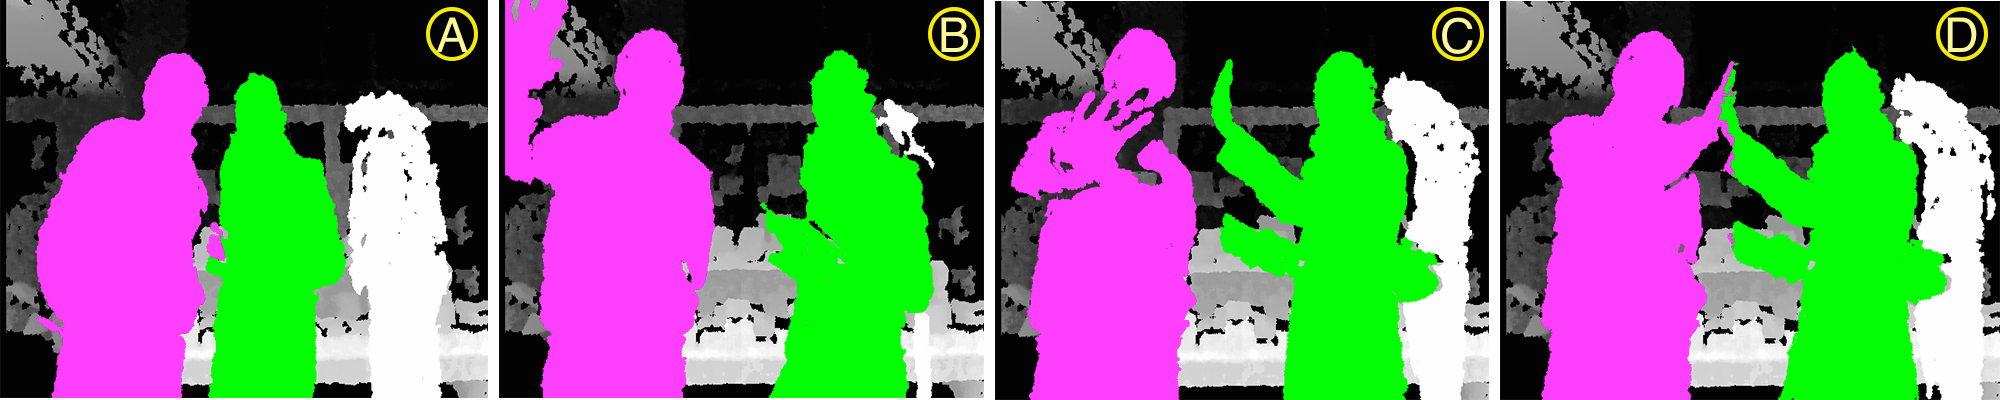
\includegraphics[width=\textwidth,height=30mm]{Figures/8/body_inter_findings/effects/playing}
    \caption{Playing with silhouette}
    \label{fig:playing_interaction}
\end{figure}
\end{flushright}
\end{minipage}

\item Interactivity confirmation: \\
People who saw their selves from far distance were not sure if the screen was interactive so they started waving their hands, body or their heads to see if their silhouette reacts to their movements. Some of the people did not apparently acted but progressively came near to screen like (spying) and then left. As can be seen in bellow frames, in (A) a person notices his/her silhouette and immediately raises hands in frame (B) and his fellow friend also notices and raises hand up in (C and D).

\begin{minipage}{0.89\textwidth}
\begin{flushright}
\begin{figure}[H]
    \centering
    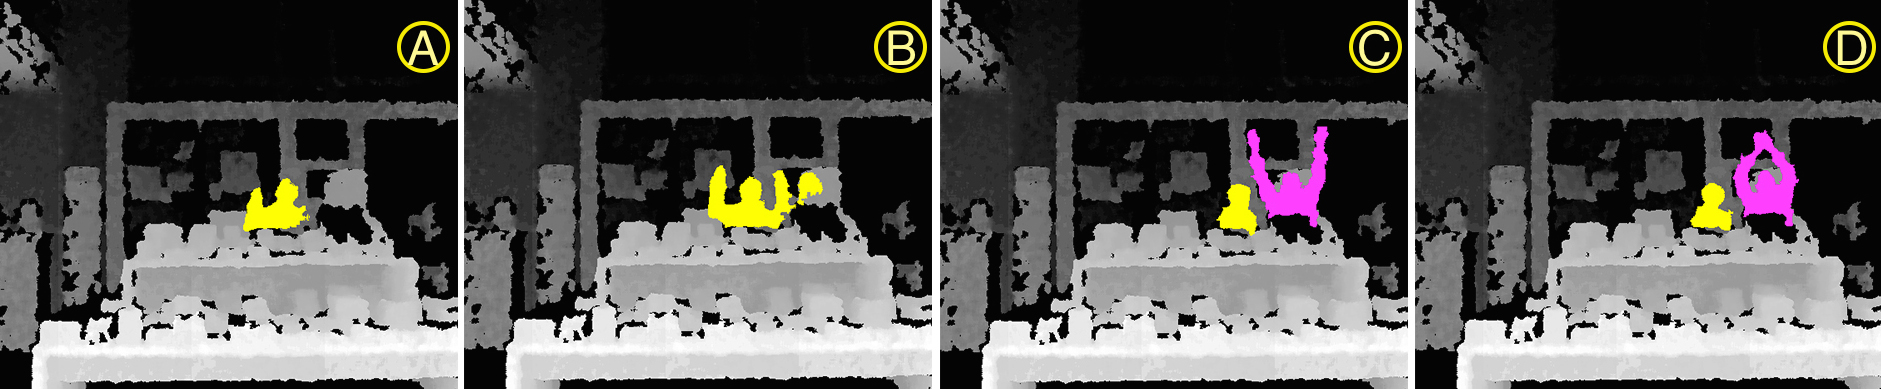
\includegraphics[width=\textwidth,height=30mm]{Figures/8/body_inter_findings/effects/noticing}
    \caption{Noticing interactivity}
    \label{fig:noticing_interactivity}
\end{figure}
\end{flushright}
\end{minipage}

\item Raising hands up: \\
During the interactions some of participants raised their hands up mainly because of the alert message that was shown on top right corner of the screen if they were undetected by Kinect camera. As can be seen in the pictures that shows different frames people during interaction and prior to interaction are raising their hands up. 


\begin{minipage}{0.89\textwidth}
\begin{flushright}
\begin{figure}[H]
    \centering
    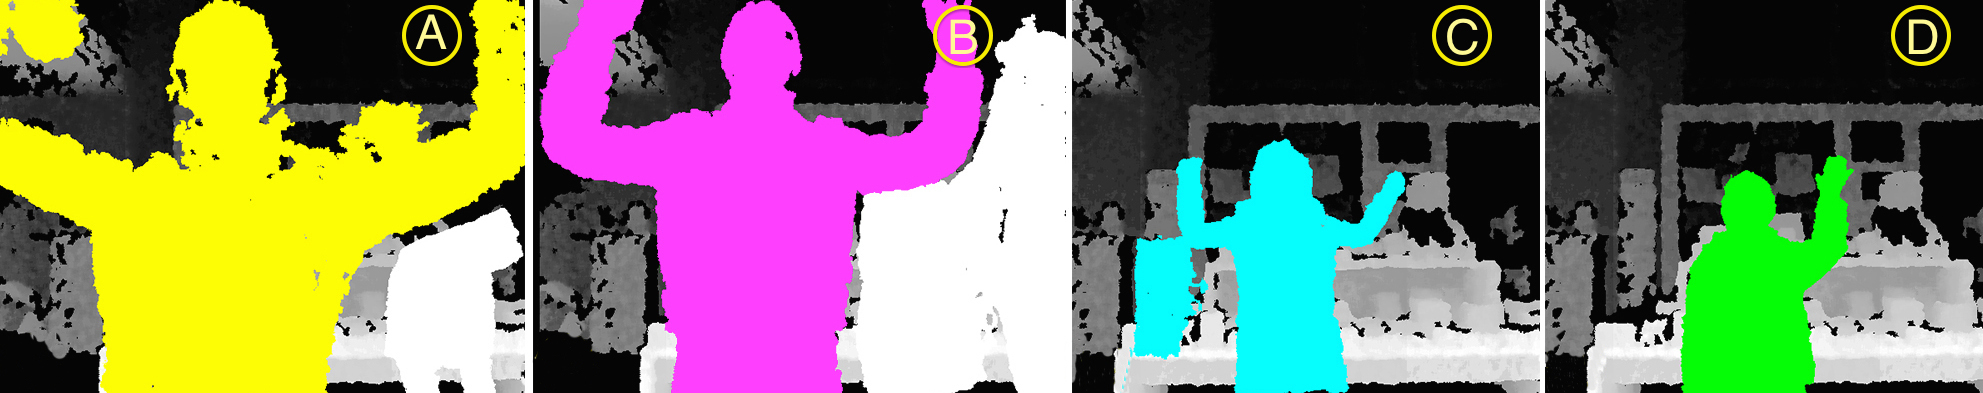
\includegraphics[width=\textwidth,height=30mm]{Figures/8/body_inter_findings/effects/raisinghand}
    \caption{Raising hand}
    \label{fig:raisinghand_interactivity}
\end{figure}
\end{flushright}
\end{minipage}

\item Physical space domination \\
The people in front of the display were either interacting or either leaving the space by walking away or turning their face back from display, people felt some sort of influence of their presence in front of it. 

\item Call-to-action reaction \\
Most people came very close to the screen when approached by the application, this lead to confusion later in interaction because the camera could not longer track them.

\item Interactions behaviors \\
The movement of silhouette during interaction is by moving forward / backward or left / right, some at early interaction leaned down or jumped higher to go forward or backward on the map.


\item Incorrect expectations \\
Some passers-by who started the interaction using their body, expected that the screen should be working using touch, they tried many times to touch the elements, one of the main reason of this behavior seemed to relied on the fact that they were called to come near, and they felt became more personal with the display and the display which was small in dimension also provides the hint of being personal. Touch interaction is know to be more personal action than using body or other gestures. 


\item Interaction negligence (technology skeptical) \\
Some of the elder participants ignored the interaction even after understanding the call-to-action, and after interviewing them they responded that they did not know how that thing works, and after interviewing an employee of the tourist information, he said that the elders are a bit skeptical about the use of technology. 

\end{itemize}

\end{enumerate}







\newpage
\subsection{Mobile Interactive findings}

\begin{enumerate}

\item Attention Level measurements \\
Attention attraction technique was quite similar to body interaction technique, which was projection passers-by silhouette but with a difference of access information text rendered on top, people would partially see their silhouette but still it was an attention mechanism, the measurement was done for five days each day for only two hours of direct observation. 


\begin{figure}[H]
    \centering
    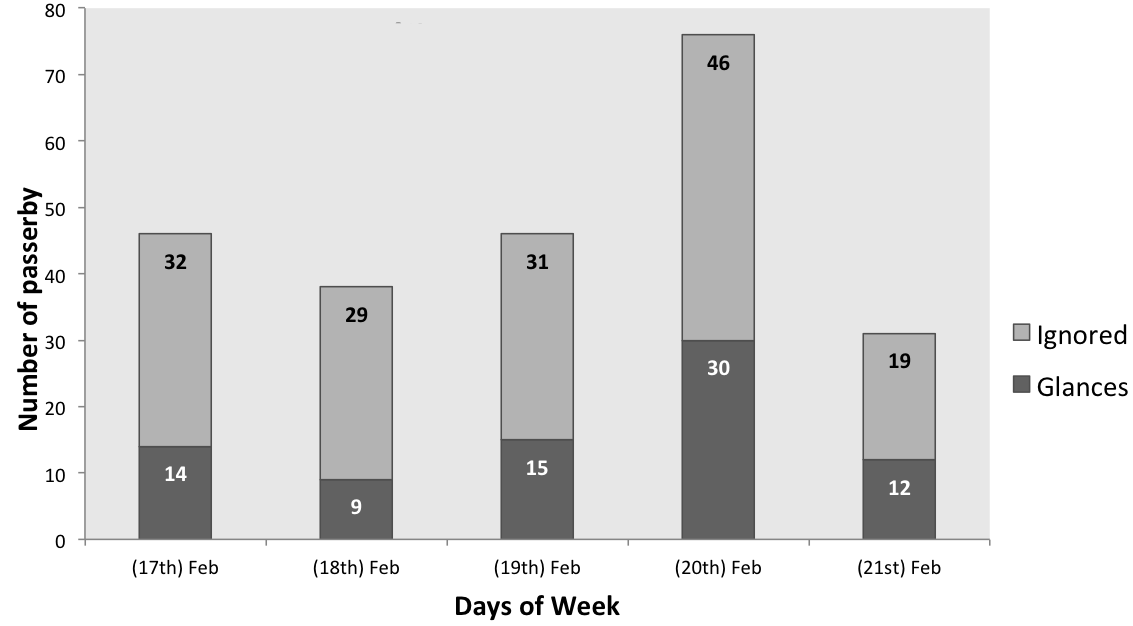
\includegraphics[width=0.9\textwidth,height=6.5cm]{Figures/8/mobile_inter_findings/mobile_Inter_chart}%
    \caption{Mobile interactive attention level chart}%
    \label{fig:mobileattentionlevelchart}%
\end{figure}

As can be seen the number of glances have decreased compared to body interaction, since other things were not changed except for the access information so it could be the result of that, that people have not fully seen themselves or recognized. 

\begin{figure}[H]
    \centering
    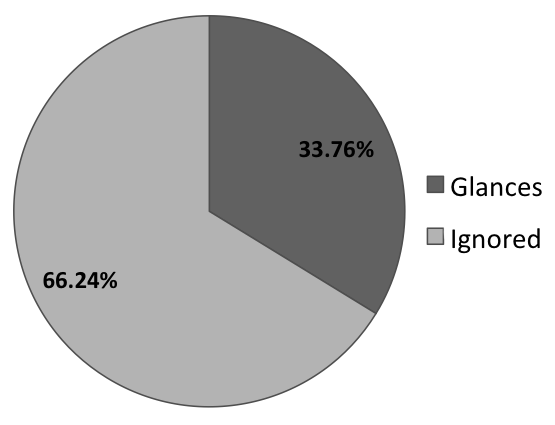
\includegraphics[width=0.45\textwidth,height=5cm]{Figures/8/mobile_inter_findings/mobile_inter_percentage}
    \caption{Attention level percentage}%
    \label{fig:bodyattentionlevelpercentage}%
\end{figure}
The percentage of the whole week of glances was around \%34 and \%66 of the cases the screen was ignored.

\newpage
\item \textbf{Engagement time} \\
Although no passers-by interacted with the system, all of the participants were in the first screen of the advertisement that showed the Bauhaus-walk name and their silhouette. It took in average around 22 seconds to be engaged passively with the screen, which is less than non-interactive and body interactive applications. 


\item \textbf{Passerby and engagements} \\
The entire five days were observed using the depth recordings and manually the number of passers-by were counted and from which the passers-by who stood for more than 3 seconds were flagged as engaged, as can be seen bellow in pie chart that shows one day each. Most of the passers-by stood for a very short time. 

\begin{figure}[H]
    \centering
    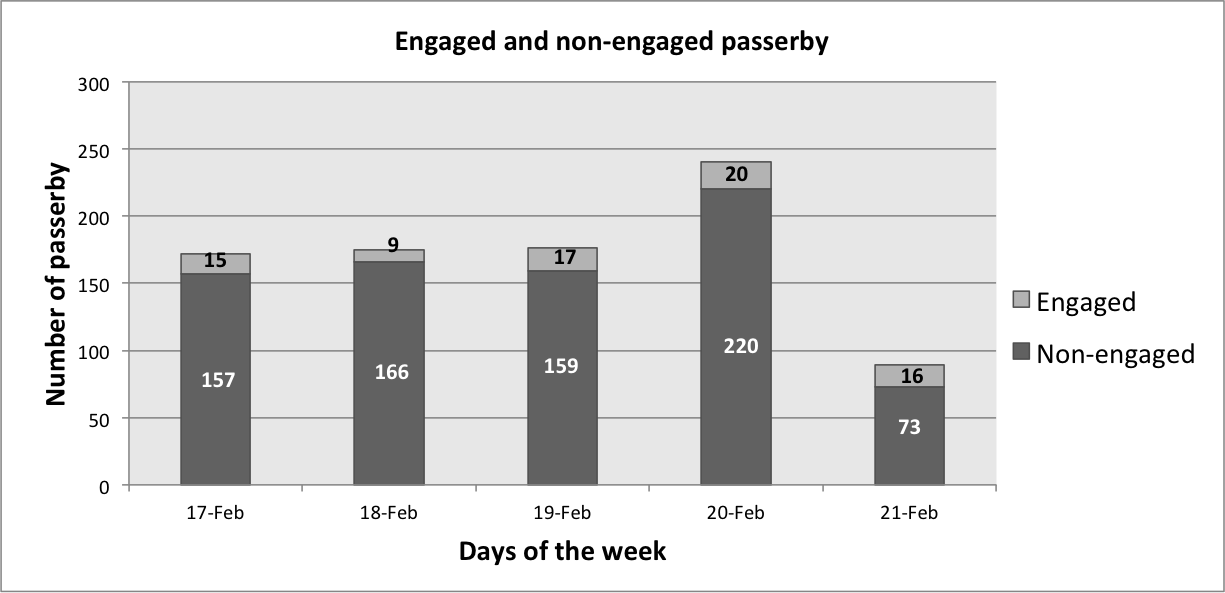
\includegraphics[width=0.9\textwidth,height=6.5cm]{Figures/8/mobile_inter_findings/mobile_inter_engage_day}
    \caption{Mobile interactive Number of engaged passerby}%
    \label{fig:mobileengagedandengagedby}%
\end{figure}


\begin{figure}[H]
    \centering
    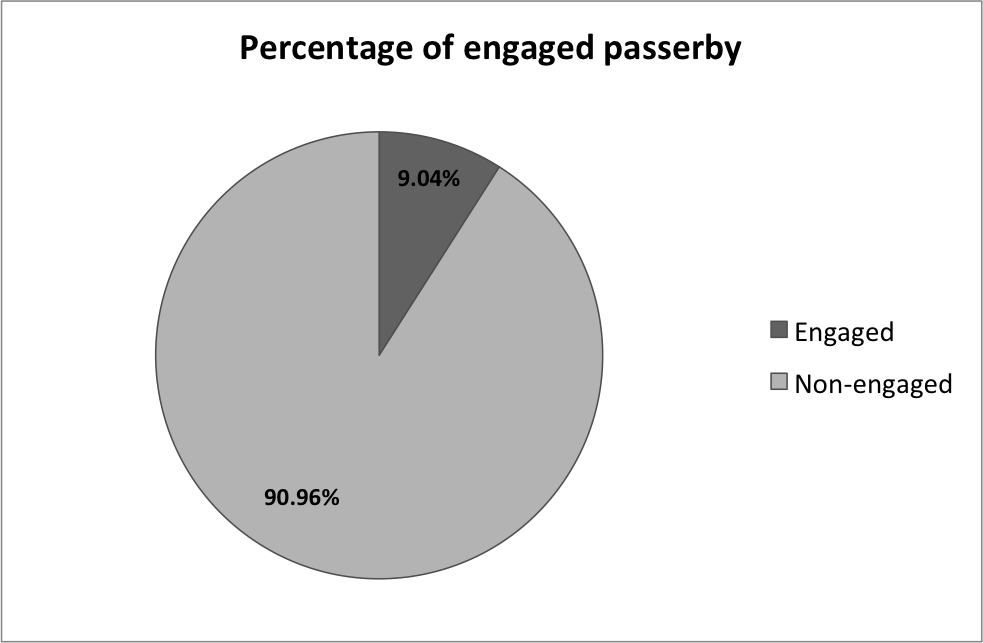
\includegraphics[width=0.45\textwidth,height=4.5cm]{Figures/8/mobile_inter_findings/mobile_eng_percentage}
    \caption{Percentage of engaged passerby}%
    \label{fig:mobileengagedpasserbypercentage}%
\end{figure}

The pie chart above illustrates that only \%9 of the passers-by were engaged with the system.


\item \textbf{Landing and Honeypot effects}
\end{enumerate}

Landing and honeypot effects in this technique were very not strong enough mainly because no passers-by interacted with the system.

Honeypot effect was mainly because of the silhouette representation as said before this effect was very week because of info-screen showed partial body representation, passers-by rarely noticed the text. Only two times honeypot effect occurred and people did not get engaged with the system afterward. This effect could have been improved if passers-by had actively participated to play game.  The picture bellow shows a green colored person at frame (A) at this point he was watching the screen for a while and when he moves out of the screen (B, C) another yellow colored person appears from the back side (C) and walks toward the screen (D, E) and gets close very close at frame (F).

\begin{minipage}{0.95\textwidth}
\begin{flushright}
\begin{figure}[H]
    \centering
    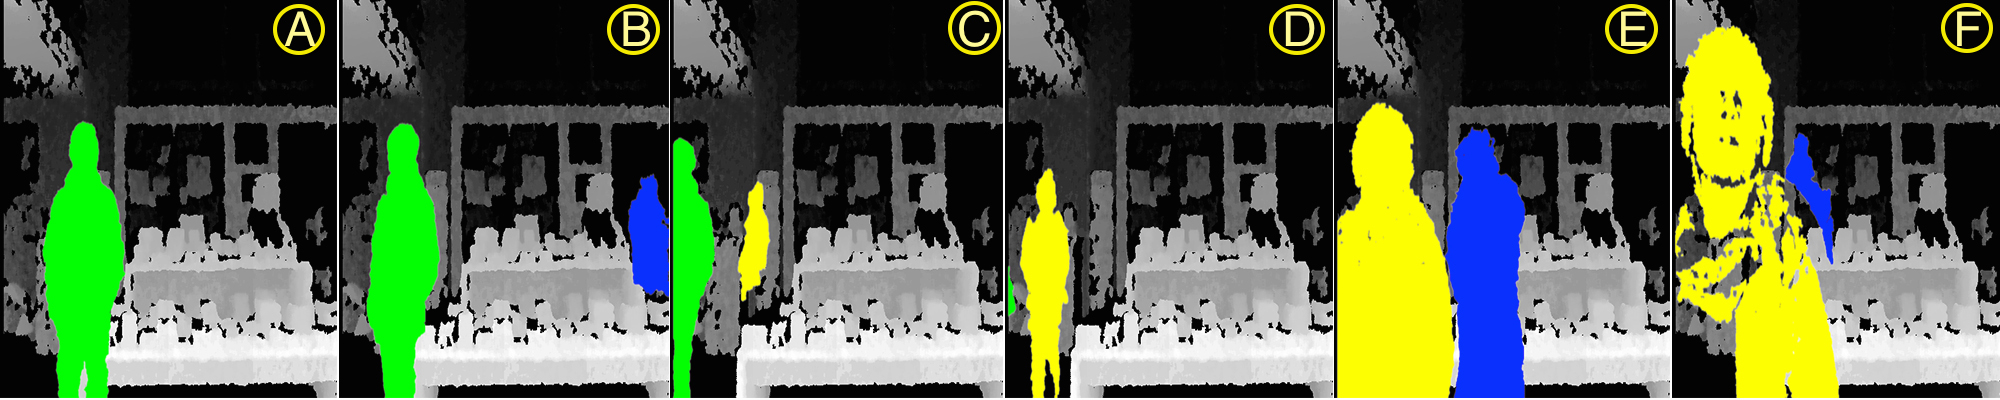
\includegraphics[width=\textwidth,height=30mm]{Figures/8/mobile_inter_findings/effects/honeypot}
    \caption{Honeypot effect}
    \label{fig:mobile_honeypoteffect}
\end{figure}
\end{flushright}
\end{minipage}


Landing effect was also recorded in some occasions and happened because they saw their silhouette, very less people noticed and most ignored. As shown in the picture from right to left a person is crossing the screen (A – E) but on frame (F) stops and move a little back to see what is on the screen. The person does not entirely come in the center of the screen. The passers-by left after standing in front of the screen without any interaction.

\begin{minipage}{0.95\textwidth}
\begin{flushright}
\begin{figure}[H]
    \centering
    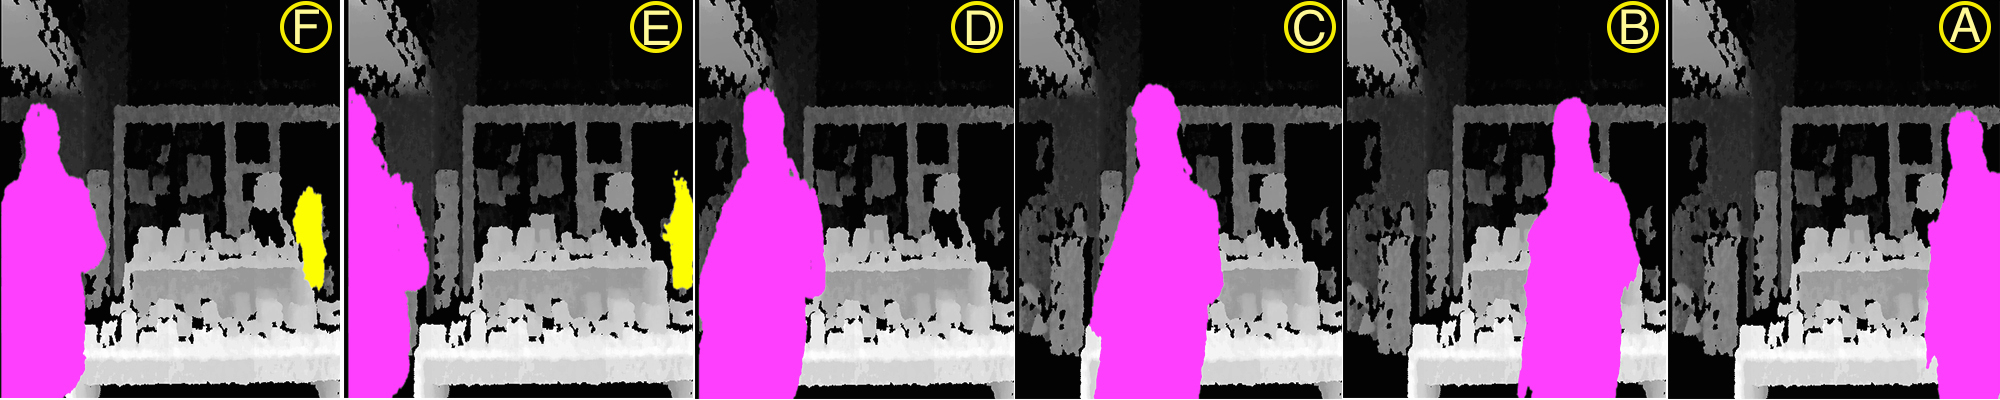
\includegraphics[width=\textwidth,height=30mm]{Figures/8/mobile_inter_findings/effects/landing}
    \caption{Landing effect}
    \label{fig:mobile_landingeffect}
\end{figure}
\end{flushright}
\end{minipage}



The bellow table shows the number of honeypot and landing effects that happened during the five days.

\begin{table}[H]
\caption{Mobile Interactive Landing and honeypot effect}
\label{tab:landingandhonypot_mobile}
\centering
\resizebox{8cm}{1.5cm}{
\begin{tabular}{| l | c | c |}
\toprule
\tabhead{Days} & \tabhead{Landing effect} & \tabhead{Honeypot effect} \\
\midrule
\textbf{17 Feb}  & 0 &  1 \\
\textbf{18 Feb}  & 1 &  0 \\
\textbf{19 Feb}  & 2 &  0 \\
\textbf{20 Feb}  & 0 &  0 \\
\textbf{21 Feb}  & 1 &  1 \\
\bottomrule
\end{tabular}
}
\end{table}



\begin{enumerate}
\setcounter{enumi}{4}

\item \textbf{Interviews}

\hilight{complete the interview report}


\newpage
\item \textbf{Other observations}

\hilight{fix Appendix and put some picture frames}
%\ref{AppendixD}.11}

Passers-by were attracted to the system when they saw their silhouette, which was kind of similar to the body interaction technique. The bellow are behaviors people had with the system.

\begin{itemize}
\item Curiosity \\
Passers-by who noticed showed curiosity and tried to come near to the screen or started waving their hands toward the screen.
 

\item Playful   \\
Most of the kids that noticed, felt excited only to see their different colored silhouette and even at some point started to dance in group. 


\item Interaction ignoring \\
All the people who were attracted ignored to interact, that could have many different reasons, like the lack of enough knowledge of how to do, or not having mobile phones or not interested to play, as one of them were interviewed he said that he does not use phone in public he only uses it for calling. 

\item Scanning code \\ 
During five days only two persons tried to scan the QR-code and after scanning they just left.


\iffalse
\item Inappropriate physical space \\
Because most of the passers-by pass and do not expect interaction with the displays and especially with mobile phone would be very difficult to be convinced because the screen is situated in the pathway of people, people would not interact with phone standing. I believe for mobile interaction it would be nice to place display where people can sit and interact.

\item Limited time \\
Passers-by have limited time to pass the screen and by mean time they should be convinced to start interaction, but as found out in the usability testing of mobile phone in previous chapter, it take much longer to understand how to start the game, this results to ignore the interaction with the smartphone. 

\item Being skeptical \\
The old generation are most of them skeptical about using technology and specially things that are their own like mobile phones, even though having a smartphone they do not tend to use their phone for public use and in this case for an advertisement. 

\item Feeling unsecure \\
Some people may thing unsecure of using their personal phone, thinking that maybe other information may be extracted from their phones, so they try to stay away from using their phones in public space. 

\fi

\end{itemize}

\end{enumerate}


\newpage
\subsection{Comparison of advertisements}
This section compares different findings of each condition as listed bellow one by one. 

\subsubsection {Number of passers-by}
Advertisements techniques were not conducted in the same days, this could ruin comparison of them in between because maybe different number of passers-by have passed in those weeks, therefor, there was a need to first compare the number of passers-by and prove that they were not statistically different in between. \\

\textbf{Hypothesis:}
\begin{itemize}
\item \textbf{H0:} There was no difference between numbers of passerby of each conditions.
\item \textbf{H1:} There was a difference between numbers of passerby of each conditions.
\end{itemize}

The bellow is the table of passerby for three weeks.

\begin{table}[H]
\caption{Number of passerby in three weeks}
\label{tab:passerbyofthreeweeks}
\centering
\resizebox{10cm}{2cm}{
\begin{tabular}{| l | c | c | c |}
\toprule
\tabhead{Days} & \tabhead{Non-interactive} & \tabhead{Body} & \tabhead{Mobile} \\
\midrule
Day 1  & 232 & 178 &  172 \\
\midrule
Day 2  & 170 & 220 &  175 \\
\midrule
Day 3  & 212 & 259 &  176 \\
\midrule
Day 4  & 209 & 216 &  240 \\
\midrule
Day 5  & 208 & 122 &  89  \\
\midrule
\textbf{Total}  & 1031 & 995 & 852 \\
\bottomrule
\end{tabular}
}
\end{table}

ANOVA test revealed that there is no significant different of passers-by between each of the conditions.\emph{(F2,5)=0.8873, p >.05 (p=0.437)}
So based on this the \emph{H0} hypothesis is being accepted and \emph{H1} hypothesis is being rejected. This gives us confidence to proceed our comparisons.

To find how small was the difference between the weeks, the eta squared(${\eta}^2$), which is an effect size index for \emph{ANOVA}, in which the $SS_{effect}$ (sum of squared) between conditions is divided by $SS_{total}$  (sum of total) as bellow.
\[
{\eta}^2 = \frac{{SS}_{effect}}{{SS}_{total}} = \frac{7293.3332}{42506.9332} = 0.1716\approx 0.18
\]

The 0.18 value means that \%18 was the difference between the weeks, which is relatively small amount of percentage and is not a matter of concern, and as a result there was no statitically difference between numbers of passers-by of each conditions between the weeks.




\subsubsection {Attention Level Comparison}
As can be seen Non-interactive had \%28.83 number of glances, the Body-interaction had almost \%10 high number of glances (\%38.70) than non-interactive, The mobile Interaction had higher glances (\%33.75) from non-interactive but still less than body interaction.  With this I can not conclude that body interaction had higher until it statistically proven.

To compare which of the the three methods drove more passers-by attention, the data of number of glances for each of the weeks were gathered as bellow and first Chi square test were applied to find if they were statistically different or not.\\

\textbf{Hypothesis: }
\begin{itemize}
\item \textbf{H0:} There was no difference between numbers of passerby of each condition.
\item \textbf{H1:} There was a difference between numbers of passerby of each condition.
\end{itemize}

% table
\begin{table}[H]
\caption{Cross tabulation for each week attention level }
\label{tab:crosstabulationweeks}
\centering
\resizebox{10cm}{2cm}{
\begin{tabular}{| l | c | c | c |}
\toprule
\tabhead{Methods} & \tabhead{Glanced (\%)} & \tabhead{Ignored} & \tabhead{Total } \\
\midrule
\textbf{Non-interactive}     & 111(\%28.83)   &   274      &   385\\
\midrule
\textbf{Body interactive }   & 106 (\%41.41)   &   150      &   256\\
\midrule
\textbf{Mobile interactive } & 80 (\%33.75)   &   157      &   237\\
\midrule
\textbf{Total }         & 297 & 581      &   878\\
\bottomrule
\end{tabular}
}
\end{table}


The Chi-squared test reveals that ${\chi}^2$\emph{(2, N=878)=10.863, p < .05 (p=.004376)},meaning that there is a difference so \emph{H0} is rejected and \emph{H1} hypothesis would be accepted.
To find that where actual difference was, each pairs were tested in between using again Chi-squared test.

\begin{enumerate}
\item Non-Interactive Vs Body Interactive \\
The finding shows that body interactive advertisement had significant number of glances than non-interactive advertisement. \\
${\chi}^2$\emph{(1, N=641)=10.863, p < .05 (p=.00437653)}

%The \emph{r-based} effect size was calculated using \emph{polyu}\footnote{Polyu: \url{http://www.polyu.edu.hk/mm/effectsizefaqs/effect_size_equations2.html}, last accessed 15 jun 2016}, and r


\item Non-Interactive Vs Mobile Interactive  \\
The finding suggests that there was no significant difference between Non-interactive and mobile in this case.\\
${\chi}^2$\emph{(1, N=622)=1.6716, p > .05 (p=.196039)}

\item Body interactive Vs Mobile Interactive \\
As can be expected the glances was not statistically significant among the body and mobile interactive advertisement too.\\
${\chi}^2$\emph{(1, N=493)=3.0663 , p > .05 (p=.07993)}

\end{enumerate}


\subsubsection {Engaged and Non-engaged passers-by}
This test is to compare if there was a difference between number of Engaged passers-by or not between the conditions.

\textbf{Hypothesis: }
\begin{itemize}
\item \textbf{H0:} There was no difference between the numbers of Engaged passers-by between the conditions.
\item \textbf{H1:} There was a difference between the numbers of Engaged passers-by between in each conditions.
\end{itemize}

The bellow table lists all number of engaged and non-engaged passers-by for three weeks.


\begin{table}[H]
\caption{Number of engaged passers-by in three weeks}
\label{tab:engagedofthreeweeks}
\centering
\resizebox{8cm}{1.5cm}{  
\begin{tabular}{| l | c | c | c |}
\toprule
\tabhead{Days} & \tabhead{Non-interactive} & \tabhead{Body} & \tabhead{Mobile} \\
\midrule
\textbf{Day 1}  & 16 & 25 &  15 \\
\midrule
\textbf{Day 2}  & 18 & 21 &  9 \\
\midrule
\textbf{Day 3}  & 15 & 26 &  17 \\
\midrule
\textbf{Day 4}  & 15 & 20 &  20 \\
\midrule
\textbf{Day 5}  & 15 & 23 &  16  \\
\midrule
\textbf{Total}  & 79 & 115 & 77 \\
\bottomrule
\end{tabular}
}
\end{table}

To determine that whether there were any significant differences between the means of these three conditions (groups), I conducted \emph{one-way ANOVA} test, and it strongly suggests that there was a significant differences of the number of Engaged passers-by between these three conditions,
 \emph{(F2,5)=11.20, p <.05 (p=.002)}.

To find where were the main difference between them, \emph{Posh-Hoc} test was carried out, the Post-Hoc Tukey’s HSD would likely identify which of the pairs of conditions were significantly different from each other. The critical value of the Studentized Range Q statistic was computed as , ${Q}_{critical}^{\alpha=0.01,k=12}$ =5.0430, and the significance can be determined if each pair’s critical value(Tukey HSD Q statistic) is bigger than Studentized Range Q statistic. ${Q}_{j}^{i }$ > ${Q}_{critical}$, and the strength of difference is determined by the \emph{P} value as shown bellow.



\begin{table}[H]
\caption{Post-Hoc Tukey’s HSD}
\label{tab:engage-non-posthoctukey}
\centering
\resizebox{\textwidth}{!}{  
\begin{tabular}{| l | c | c | c |}
\toprule
\tabhead{Methods} & \tabhead{Tukey HSD Q statistic} & \tabhead{Tukey HSD p-value} & \tabhead{Tukey HSD inferfence} \\
\midrule
\textbf{A vs B}  & 5.6337 & 0.0047509 &  ** p<0.01  \\
\midrule
\textbf{A vs C}  & 0.3130 & 0.8999947 &  insignificant \\
\midrule
\textbf{B vs C}  & 5.9467 & 0.0032197 &  ** p<0.01 \\

\bottomrule
\end{tabular}
}
\end{table}

Method A, B and C refers to (Non-interactive, body interactive and mobile interactive) advertisement accordingly. As can be seen from the above chart, there is no significant difference between group A and C because the critical value is not bigger than 5.0430 and also the \emph{p} value is bigger than 0.5, but group B shows a significant difference between A and C because the critical value is higher than 5.0430, and the \emph{p} is smaller than 0.01. It shows that the body interactive advertisement engaged significantly more passers-by than other two types of advertisement.

To find out how big is the difference between engaged passers-by in non-interactive and body interactive conditions, the eta squared(${\eta}^2$), which is an effect size index for \emph{ANOVA}, in which the $SS_{effect}$ (sum of squared) between conditions is divided by $SS_{total}$  (sum of total) as bellow calculated by online tool \emph{Easycalculator}\footnote{easycalculator: \url{https://www.easycalculation.com/statistics/eta-square-calculator.php}, last accessed 15 jun 2016}.
\[
{\eta}^2 = \frac{{SS}_{effect}}{{SS}_{total}} = \frac{129.6}{162.4} = 0.798 \approx 0.8
\]

The 0.8 means that \%80 of total variance is accounted for by the conditions (body interactive, non-interactive) effect. 


\subsubsection {Landing effect}
The bellow table shows how many landing effects were recorded from the depth observation video for each of the weeks.\\


\textbf{Hypothesis: }
\begin{itemize}
\item \textbf{H0:} There was no difference between the number of landing effect of Passers-by for each condition.
\item \textbf{H1:} There was a difference between the number of landing effect of Passers-by for each condition.
\end{itemize}

\begin{table}[H]
\caption{Number of Landing effect in three weeks}
\label{tab:landingeffectthreeweeks}
\centering
\resizebox{8cm}{1.5cm}{  
\begin{tabular}{| l | c | c | c |}
\toprule
\tabhead{Days} & \tabhead{Non-interactive} & \tabhead{Body} & \tabhead{Mobile} \\
\midrule
\textbf{Day 1}  & 1 & 2 &  0 \\
\midrule
\textbf{Day 2}  & 0 & 3 &  1 \\
\midrule
\textbf{Day 3}  & 2 & 2 &  2 \\
\midrule
\textbf{Day 4}  & 0 & 2 &  0 \\
\midrule
\textbf{Day 5}  & 1 & 3 &  1  \\
\bottomrule
\end{tabular}
}
\end{table}

ANOVA test reveals that there was a significant difference between one or two above conditions, ( \emph{(F2,5)=7.5294, p <.05 (p=.0076)}). So I reject the Null hypothesis and state that one or more of the above conditions were statistically different from the others, 

To confirm that which of the pairs were different significantly, I run Post-Hoc Tukey’s HSD test, the critical value of the Studentized Range Q statistic was computed as , ${Q}_{critical}^{\alpha=0.05,k=12}$ =3.7711, and the significance can be determined if each pair’s critical value(Tukey HSD Q statistic) is smaller than Studentized Range Q statistic. ${Q}_{j}^{i }$ > ${Q}_{critical}$, and the strength of difference is determined by the \emph{P} value as shown bellow.

\begin{table}[H]
\caption{Post-Hoc Tukey’s HSD results}
\label{tab:landing-non-posthoctukey}
\centering
\resizebox{\textwidth}{!}{ 
\begin{tabular}{| l | c | c | c |}
\toprule
\tabhead{Methods} & \tabhead{Tukey HSD Q statistic} & \tabhead{Tukey HSD p-value} & \tabhead{Tukey HSD inferfence} \\
\midrule
\textbf{A vs B}  & 4.7527 & 0.0144554 &  * p<0.05  \\
\midrule
\textbf{A vs C}  & 0.0000 & 0.8999947 &   insignificant \\
\midrule
\textbf{B vs C}  & 5.9467 & 0.0144554 &  * p<0.05 \\

\bottomrule
\end{tabular}
}
\end{table}


Group A, B and C refers to (Non-interactive,body interactive and mobile interactive) advertisement accordingly As can be seen the test shows that the condition A and C were insignificant but condition B is significant from A and C, which means that body interactive advertisement has statistically higher landing effects than other two conditions.

To find out how big is the difference between number of landing effects in non-interactive and body interactive conditions, the eta squared(${\eta}^2$), which is an effect size index for \emph{ANOVA}, in which the $SS_{effect}$ (sum of squared) between conditions is divided by $SS_{total}$  (sum of squared )total as bellow calculated by online tool \emph{Easycalculator}\footnote{easycalculator: \url{https://www.easycalculation.com/statistics/eta-square-calculator.php}, last accessed 15 jun 2016}.
\[
{\eta}^2 = \frac{{SS}_{effect}}{{SS}_{total}} = \frac{5.12}{7.84} = 0.6531 \approx 0.66
\]

The 0.66 means that \%66 of total variance is accounted for by the conditions (body interactive, non-interactive) effect.



\subsubsection {Honeypot effect}
The bellow table shows how many honeypot effects were recorded from the depth observation video for three conditions.\\

\textbf{Hypothesis: }
\begin{itemize}
\item \textbf{H0:} There is no significant difference between the numbers of honeypot effect for the conditions.
\item \textbf{H1:} There is significant difference between the numbers of honeypot effect for the conditions.
\end{itemize}


\begin{table}[H]
\caption{Number of Honeypot effect in three weeks}
\label{tab:landingeffectthreeweeks}
\centering
\resizebox{8cm}{1.5cm}{  
\begin{tabular}{| l | c | c | c |}
\toprule
\tabhead{Days} & \tabhead{Non-interactive} & \tabhead{Body} & \tabhead{Mobile} \\
\midrule
\textbf{Day 1}  & 1 & 2 &  1 \\
\midrule
\textbf{Day 2}  & 1 & 3 &  0 \\
\midrule
\textbf{Day 3}  & 2 & 2 &  0 \\
\midrule
\textbf{Day 4}  & 2 & 5 &  0 \\
\midrule
\textbf{Day 5}  & 1 & 3 &  1  \\
\bottomrule
\end{tabular}
}
\end{table}


ANOVA test reveals that there is a significant different between the conditions,(\emph{(F2,5)=12.29, p <.05 (p=.001)}), and from that I reject the null hypothesis and accept that there was a statistical difference between one of the conditions in the number of honeypot effects. To find which of the pairs were significant different the Post-hoc Tukey test was applied as bellow. 

\begin{table}[H]
\caption{Post-Hoc Tukey’s HSD results}
\label{tab:honeypot-non-posthoctukey}
\centering
\resizebox{\textwidth}{!}{ 
\begin{tabular}{| l | c | c | c |}
\toprule
\tabhead{Methods} & \tabhead{Tukey HSD Q statistic} & \tabhead{Tukey HSD p-value} & \tabhead{Tukey HSD inferfence} \\
\midrule
\textbf{A vs B}  & 4.2762 & 0.0264780 & * p<0.05  \\
\midrule
\textbf{A vs C}  & 2.6726 & 0.1836687 & insignificant \\
\midrule
\textbf{B vs C}  & 6.9488 & 0.0010053 & ** p<0.01 \\
\bottomrule
\end{tabular}
}
\end{table}

Group A, B and C refers to (Non-interactive, body interactive and mobile interactive) advertisement accordingly. Post-hoc Tukey computed the critical value (Studentized Range Q statistic) for A and B as, ${Q}_{critical}^{\alpha=0.05,k=12}$ = 5.0430 for and another  value for B and C as, ${Q}_{critical}^{\alpha=0.05,k=12}$ = 3.7711 and the significance can be determined if each pair’s critical value(Tukey HSD Q statistic) is bigger than Studentized Range Q statistic. ${Q}_{j}^{i }$ > ${Q}_{critical}$, and the strength of difference is determined by the \emph{P} value as shown above. From the diagram above it is very clear that non-interactive with mobile interactive is insignificant, but the non-interactive with body is significant and body and mobile is strongly significant too.

To find out how big is the difference between number of honeypot effects in non-interactive and body interactive conditions, the eta squared(${\eta}^2$), which is an effect size index for \emph{ANOVA}, in which the $SS_{effect}$ (sum of squared) between conditions is divided by $SS_{total}$  (sum of total) as bellow calculated by online tool \emph{Easycalculator}\footnote{easycalculator: \url{https://www.easycalculation.com/statistics/eta-square-calculator.php}, last accessed 15 jun 2016}.

\[
{\eta}^2 = \frac{{SS}_{effect}}{{SS}_{total}} = \frac{6.4}{13.6} = 0.4706 \approx 0.47
\]

The 0.47 means that \%47 of total variance is accounted for by the conditions (body interactive, non-interactive) effect. Even though they are statistically significant but the effect size is low, which makes this effect not very significant, that is why only one (*) is given in above inference column. But the comparison of body and mobile has two (*) which means that body performed much more better than mobile and is assumed to have a larger effect size.

\hilight{discusse on effect size}

\section{Discussion}

As in non-interactive, the phases were automatically triggered one after another in sequence of time, and passers-by might have encountered to different phases in different occasions and this could have influenced the attention level because not all the phases had the same interfaces, in the first phase the screen did not had enough movement and the other phases had more pictures, movements and colors, but there was a higher chance of encounters of passers-by with the second two interfaces because of the durations they were shown like, the first phase was only for 5 seconds and the others were for 20 to 40 seconds. While on other hand in interactive advertisements, passers-by had more encounters with the first phase because of the silhouette representation, this phase did not had any time limitation until the game interaction was not started.

Engagement of passers-by with the system were also different in three conditions, in non-interactive people might be engaged in watching the two phases (map and video phases) and in body-interactive in the first two phases (attraction, map phases) and in mobile interaction, the engagement was only in the first phase (attraction). Despite these difference in all the phases the Bauhaus-Walk logo and goal of the event was mentioned, people still could understand that what was the advertisement about.

Honeypot effect was more seen in interactive advertisement compared to non-interactive one of the reasons could be, \emph{Interaction movement}, passers-by perform interactions that involve body movement and the movements can attract other nearby, while in non-interactive there were very limited movement. The landing effect was also significant in interactive compared to non-interactive. One of the main reasons could be that in non-interactive passers-by could have encountered in different phases of display and some of the phases might have been interested or more attractive and they performed landing, and in other phases they might have not performed landing effect at all, while in interactive advertisement, passers-by had performed landing effect in the first phase (silhouette representation) and in this case also not all had landed back to screen some people might have liked it and some might not.

In body interactive advertisement, People did not stayed longer than 4.61 seconds to watch the video, which is very less compared to the interactive phases (game, silhouette). There could be many reasons for this, (1) \emph{interaction disturbance}, The video phase is a disturbance to participants interaction and I believe that no one likes to be disturbed while they are busy with something, (2)\emph{End of Fun}, by showing the ad video, the participant loses that interest and enjoyments while he/she had during the interaction, (3) \emph{dis-connectivity}, the person feels disconnected to the screen and there is no more place for him/her in display, (4) \emph{Force to watch}, the person feels the direct force to watch the advertisement video, (5) \emph{Time consuming}, participant might think that it will take time to watch till the end of video  (6)\emph{Traditional ad effect}, it has the feeling of traditional TV or radio advertising like, in the middle of a movie an advertising video is shown, which people often do something else till the movie start again.
\hilight{to play come close, is missleading}


In Mobile interactive advertisement no one interacted with the game using their mobile phone, this could have many reasons, (1) \emph{feel of Insecurity and trust}, smartphones are used by people for calling, messaging, note-taking, emailing, videoing, photographing and for other personal usages, therefor people feel insecure to use their smartphones in public spaces so that their personal belonging might not be theft by other people, in this case the owner of the advertising screen, (2)\emph{Limited technical knowledge}, not all people have technical knowledge about the use of smartphone, specially the elder people, who can only use it for calling or texting, but not connecting to internet or playing games, (3) \emph{Lack of smartphones}, elder people still use their old mobile phones, which does not have Wi-Fi or browser capabilities, (4) \emph{Physical setup}, the screen was placed in pathway, where people walk often, there is not a comfortable area to sit, connect to system and interact with the game, (5) \emph{Time consuming}, the use of phone and specially a game is considered to be time consuming process, and people in Tourist information center do not have that much time to take their phone and play, (6) \emph{Confusion}, the attraction method was with the use of body silhouette representation, and the interaction was with mobile phone, which might have confused passers-by. 


\section{Conclusion}
This chapter concludes the findings and observations of three different advertisement techniques from which one was non-interactive and two of the others were interactive as described bellow.

Non-interactive advertisement in tourist information was very quite, people reacted normally, the sense of joy and excitement was not felt with display, participants selectively stood and read the advertisement for a short period of time and most of others ignored the displays, around 1/4 passers by glanced in each two hours of observation, \%7.6 passers-by were engaged among all the passers-by in the entire days of week and spent 34 seconds in average, people liked the design of the interface, but also complained about the speed and theme of content.

Body interactive advertisement started with joy and fun, the behavior toward the screen was different from the non-interactive, attention level was about \%41.41 that passers-by glanced toward display, and people among all passers-by during the week \%12 of them were engaged that took 42 seconds in average.

Many landing effects and honeypot effects were observed and beside that, people reacted differently to notice the interactivity and approached toward the screen, the interactions happened individually and in groups, the attraction attention method was appreciated and participants understood how to trigger the interaction mode. In this technique a lot of passers-by seemed to be active at front of the monitor, the physical space around the screen directly had influenced the people behaviors, people called other friends to join the interaction and raised a sense of awareness around. 

Mobile interaction technique was one of techniques that did not really find its value in the environment, except for the attraction attention area, no one interacted with the system and no one were motivated to try at-least for one time, but still people were interested to see their silhouette and spent a little time in front of the display. \%33 of passers-by glanced and among all passers-by during the week only \%9 of them were engaged within 22 second in average.

At the conclusion from the findings and observations and comparisons of all three different techniques body interaction technique was the most statistically attractive, which received higher number of glances, increased the number of whole passers-by to be engaged, increased the duration of engagement and raised number of honeypot and landing effects. This technique was one of the most acceptable and preferred techniques for interaction in the area by participants. The use of ad video after body interaction is not suitable for interaction design, else participants would leave the interaction quickly, The video could be embedded inside the interaction phase for a short period of time should not occlude the silhouette so that the person do not feel disconnected with the advertisement. The non-interactive and mobile interactive findings were not significant and I believe that mobile interactive advertisement would be significant if it is installed in a location that is comfortable for people to sit and take time to interact and the target audience should be more from young generation, who are more familiar with the technologies.